\documentclass[12pt,a4paper]{amsart}

\usepackage[T1]{fontenc}
\usepackage[utf8]{inputenc}
\usepackage[british]{babel}
\usepackage{mathtools}
\usepackage{amssymb}
\usepackage{mathrsfs}
\usepackage{enumitem}
\usepackage{tikz-cd}
\usetikzlibrary{decorations.markings}
\usepackage{float}
\usepackage{hyperref}
\urlstyle{same}
\usepackage[noabbrev]{cleveref}

\theoremstyle{plain}
\newtheorem{thm}{Theorem}[section]
\newtheorem{thmdefn}[thm]{Theorem-Definition}
\newtheorem{lm}[thm]{Lemma}
\newtheorem{prop}[thm]{Proposition}
\newtheorem{cor}[thm]{Corollary}
\theoremstyle{definition}
\newtheorem{defn}[thm]{Definition}
\newtheorem{exmp}[thm]{Example}
\newtheorem{xca}[thm]{Exercise}
\theoremstyle{remark}
\newtheorem{rem}[thm]{Remark}
\Crefname{thm}{Theorem}{Theorems}
\Crefname{thmdefn}{Theorem-Definition}{Theorem-Definitions}
\Crefname{lm}{Lemma}{Lemmas}
\Crefname{prop}{Proposition}{Propositions}
\Crefname{cor}{Corollary}{Corollaries}
\Crefname{defn}{Definition}{Definitions}
\Crefname{exmp}{Example}{Examples}
\Crefname{xca}{Exercise}{Exercises}
\Crefname{rem}{Remark}{Remarks}

\title[Notes on enumerative geometry]{Notes on enumerative geometry}
\author[Pedro N\'{u}\~{n}ez]{}
\address{Pedro N\'{u}\~{n}ez \newline
\indent Albert-Ludwigs-Universit\"{a}t Freiburg, Mathematisches Institut \newline
\indent Ernst-Zermelo-Straße 1, 79104 Freiburg im Breisgau (Germany)}
\email{\normalfont\href{mailto:pedro.nunez@math.uni-freiburg.de}{pedro.nunez@math.uni-freiburg.de}}
\renewcommand*{\urladdrname}{\itshape Homepage}
\urladdr{\normalfont\href{https://home.mathematik.uni-freiburg.de/nunez/}{https://home.mathematik.uni-freiburg.de/nunez} \newline
\mbox{ }\newline 
\indent {\fontfamily{libertine}\selectfont
I would like to thank the DFG-Graduiertenkolleg GK1821 ``Cohomological Methods in Geometry'' for their support!%
}}
\date{\today}

\setcounter{tocdepth}{1}
\sloppy
\makeatletter
\hypersetup{
  pdfauthor={\authors},
  pdftitle={\@title},
  colorlinks,
  linkcolor=[rgb]{0.2,0.2,0.6},
  citecolor=[rgb]{0.2,0.6,0.2},
  urlcolor=[rgb]{0.6,0.2,0.2}}
\makeatother
\makeatletter
\tikzcdset{
open/.code={\tikzcdset{hook, circled};},
closed/.code={\tikzcdset{hook, slashed};},
circled/.code={\tikzcdset{markwith={\draw (0,0) circle (.375ex);}};},
slashed/.code={\tikzcdset{markwith={\draw[-] (-.4ex,-.4ex) -- (.4ex,.4ex);}};},
markwith/.code={
\pgfutil@ifundefined{tikz@library@decorations.markings@loaded}%
{\pgfutil@packageerror{tikz-cd}{You need to say %
\string\usetikzlibrary{decorations.markings} to use arrow with markings}{}}{}%
\pgfkeysalso{/tikz/postaction={/tikz/decorate,
/tikz/decoration={
markings,
mark = at position 0.5 with
{#1}}}}},
}
\makeatother

\begin{document}

\maketitle

\begin{abstract}
	Notes based on the Wednesday Seminar held at Freiburg during the Winter Semester 2020/2021 and typesetted by Pedro N\'{u}\~{n}ez.
	Any errors or typos were likely introduced by myself; corrections and any other suggestions are very much appreciated!
\end{abstract}

\tableofcontents

The main reference for this seminar is the book \cite{eh16}.

\section{Ivan Zaccanelli: The Chow ring (16.12.2020)}

\subsection{Introduction}

Some instances of enumerative problems:

\begin{itemize}
    \item Given $f\in K[x]$ of degree $\deg(f)=d$, what is the cardinality of the set $\{ x\in K\mid f(x)=0\}=:V(f)$?
	\underline{Answer:} it is $d$ if the the axis $V(y)$ in the plane is not tangent to the graph of $f$, given by $V(y-f(x))$ and if $K=\bar{K}$.
	If there were some tangent intersection points we would have to take multiplicities into account.
	\[ \rightsquigarrow \text{We want to consider }K=\mathbb{C}. \]
    \item Given $f,g\in \mathbb{C}[x_{1},x_{2}]$, with $\deg(f)=d$ and $\deg(g)=e$ such that $V(f)$ and $V(g)$ ``intersect transversally'', what is the cardinality of $V(f)\cap V(g)$?
	\underline{Answer:} (Bézout) it is $d\cdot e$... if we look at this question in the projective plane $\mathbb{P}^{2}$.
	\[ \rightsquigarrow \text{We want to consider varieties in }\mathbb{P}^{n}. \]
    \item Given four lines in $\mathbb{P}^{3}$, how many lines intersect all of them?
	\underline{Answer:} postponed to 27.01.2021.
\end{itemize}

Let us now see a ``backwards proof'' of Bézout's theorem:

\begin{proof}[``Backwards proof'']
    The theorem implies that the cardinality of $V(f)\cap V(g)$ only depends on $\deg(f)$ and $\deg(g)$.
    So we can replace $f$ by $\tilde{f}$ and $g$ by $\tilde{g}$ such that $V(\tilde{f})$ is the union of $d$ lines in the projective plane and $V(\tilde{g})$ is the union of $e$ lines in projective plane.
    Moreover we can assume that these lines are in general position, thus the cardinality of the intersection is indeed $d\cdot e$.
\end{proof}

Some of the ideas that we want to make rigurous are:

\begin{itemize}
    \item ``Move'' or identify some subvarieties.
    \item Show that the cardinality of the intersection does not depend on this identification, given that the intersection is transverse.
\end{itemize}

\[ \rightsquigarrow \text{Fundamental tool: Chow ring }\operatorname{CH}^{\bullet}(X)\text{ of a quasi-projective variety } X.\]

As a side note, let us ask the following question: is such a rigurous foundation really necessary?
To answer it, let us look at some history of these kinds of problems:

\begin{itemize}
    \item Schubert ``guessed'' correctly in 1879 that the number of twisted cubics tangent to 12 quadrics is 5819539783680.
	\[ \rightsquigarrow \text{Maybe the answer is ``no'', at least not for him.} \]
	Quoting Eisenbud and Harris: ``He landed a jumbo jet being blindfolded.''
    \item Hilbert includes this issue as his 15th problem in 1900.
	\[ \rightsquigarrow \text{The answer is ``yes'' for him.} \]
    \item Fulton wrote a bible book about this in 1984 \cite{ful98}.
	\[ \rightsquigarrow \text{Just cite him whenever necessary!} \]
\end{itemize}

\subsection{Quick recap of algebraic varieties}

The Zariski topology on $\mathbb{A}^{n}$ (resp.~on $\mathbb{P}^{n}$) has as closed subsets those of the form $V(I)$ for $I\subseteq \mathbb{C}[x_{1},\ldots,x_{n}]$ an ideal (resp.~$V(I)$ for $I\subseteq \mathbb{C}[x_{0},\ldots,x_{n}]$ a homogeneous ideal.
The sheaf of regular functions consists of functions that can be locally written as a quotient of two polynomials (resp.~homogeneous polynomials).
A closed subset $X\subseteq \mathbb{A}^{n}$ (resp.~$X\subseteq \mathbb{P}^{n}$) is said to be an \textit{affine variety} (resp.~a \textit{projective variety}).

A \textit{quasi-projective variety} is an open set inside a projective variety.

\begin{defn}[Irreducibility]
    A non-empty topological space is said to be \textit{irreducible} if it cannot be written as a union of two proper closed subsets.
\end{defn}

\begin{exmp}
    The subset $V(xy)\subseteq \mathbb{A}^{2}$ is connected but not irreducible, since it can be written as
    \[ V(xy)=V(x)\cup V(y). \]
    \begin{figure}[H]
	\centering
	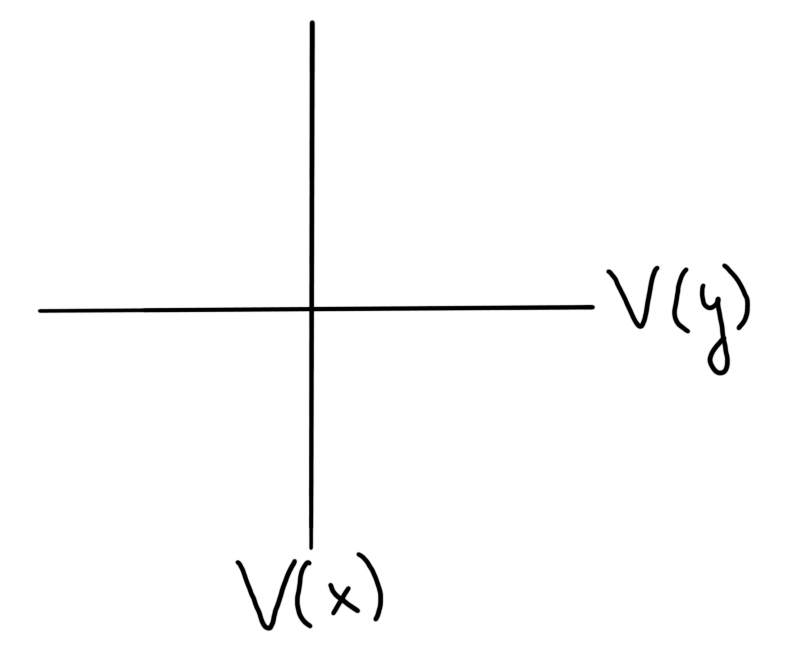
\includegraphics[scale=.15]{pictures/axes}
    \end{figure}
\end{exmp}

\begin{prop}
    Each $X\subseteq \mathbb{P}^{n}$ can be written uniquely as $X=\cup_{i=1}^{r}X_{i}$, where $X_{i}\subseteq X$ are closed and irreducible and no $X_{i}$ is superfluous.
\end{prop}

The $X_{i}$'s in the previous proposition are called the \textit{irreducible components} of $X$.

\begin{defn}[Dimension]
    The \textit{dimension} of $X\subseteq \mathbb{P}^{n}$ is defined as the maximal length of a chain
    \[ Y_{0}\subsetneq Y_{1}\subsetneq \cdots \subsetneq Y_{n}\subseteq X \]
    with each $Y_{i}$ closed and irreducible.
\end{defn}

\begin{defn}[Smoothness]
    $X\subseteq \mathbb{P}^{n}$ is \textit{smooth} if $\dim(X)=\dim(T_{p}X)$ for all $p\in X$.
\end{defn}

\underline{Bad news:} for intersection theory we must also take into account subschemes.
In the setting above, $V(I)=V(I^{2})$.
But problems arise naturally taking intersections.
In $\mathbb{A}^{2}$ we have
\[ V(y)\cap V(y-x^{2})=V((y)+(y-x^{2}))=V(x^{2},y)\overset{!}{\neq} V(x,y). \]
\begin{figure}[H]
    \centering
    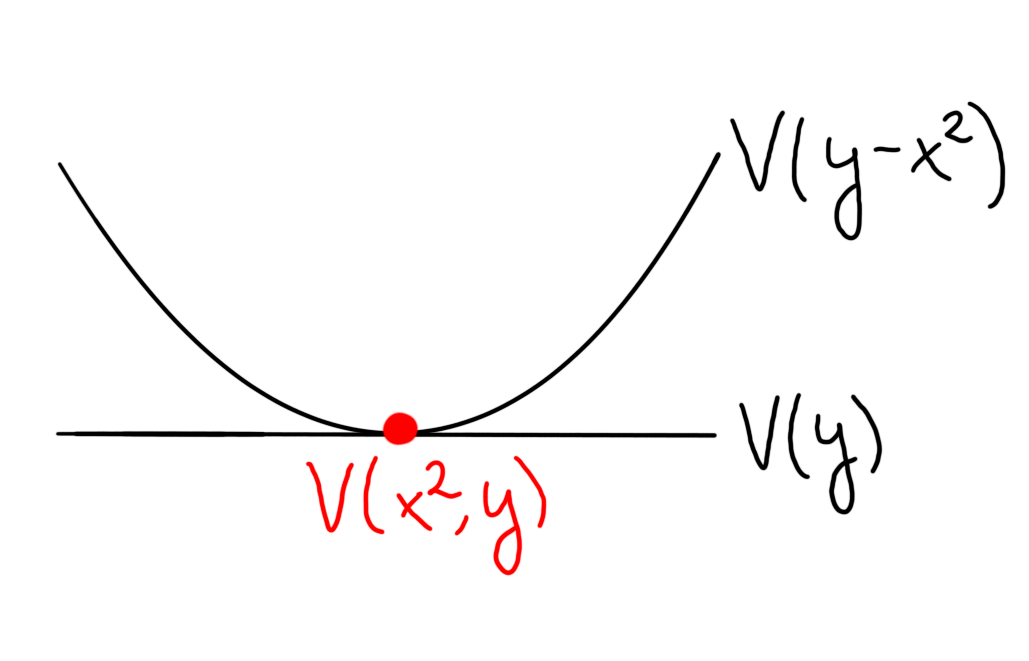
\includegraphics[scale=.15]{pictures/tangent}
\end{figure}

Moral: an (affine) subscheme is the datum of an (affine) variety together with the ideal defining it.

From now on, ``variety'' means ``irreducible variety''; and ``subvariety'' means ``irreducible closed subset in some variety''.

\subsection{Chow group}

Let $X$ be a quasi-projective variety.

\begin{defn}[Cycle group]
    The \textit{group of cycles} $Z(X)$ is the free abelian group generated by the set of subvarieties in $X$.
\end{defn}

So if we have $Y_{1},\ldots,Y_{m}\subseteq X$ closed and irreducible, then

\[ \sum_{i=1}^{m}a_{i}Y_{i} \in Z(X). \]

\begin{rem}\mbox{ }
    \begin{enumerate}
	\item $Z(X)$ is graded (as an abelian group) by the dimension or by the codimension:
	    \[ Z(X)=\oplus_{k\in \mathbb{N}}Z_{k}(X)=\oplus_{l\in \mathbb{N}}Z^{l}(X), \]
	    where $Z_{k}(X)$ denotes the subgroup generated by subvarieties of dimension $k$ and $Z^{l}(X):=Z_{\dim(X)-l}(X)$.
	\item To each subscheme $Y\subseteq X$ we can associate a cycle
	    \[ \langle Y\rangle:=\sum n_{i}Y_{i},  \]
	    where the $Y_{i}$ are the irreducible components of the support of $Y$ and the $n_{i}$ keep track of the multiplicity of each component.
    \end{enumerate}
\end{rem}

\begin{exmp}
    \[ \langle V(x^{2},y)\rangle =2V(x,y). \]
\end{exmp}

\begin{defn}[Chow group]
    We define the \textit{Chow group} of $X$ as
    \[ \operatorname{CH}(X):=Z(X)/\operatorname{Rat}(X), \]
    whee $\operatorname{Rat}(X)$ is the subgroup generated by cycles of the form
    \[ \langle \Phi\cap (\{t_{0}\}\times X)\rangle - \langle \Phi\cap (\{t_{1}\}\times X)\rangle, \]
    where $\cap$ denotes the scheme-theoretic intersection, $t_{0},t_{1}\in \mathbb{P}^{1}$ and $\Phi\subseteq \mathbb{P}^{1}\times X$ is a subvariety not contained in any fiber $\{t\}\times X$.
\end{defn}

If $Z_{1},Z_{2}\in Z(X)$ are cycles such that $[Z_{1}]=[Z_{2}]$, then we say that they are \textit{rationally equivalent} cycles.

\begin{exmp}\mbox{ }
    \begin{enumerate}
	\item In $\mathbb{P}^{1}$, any two points are rationally equivalent:
	    \begin{figure}[H]
		\centering
		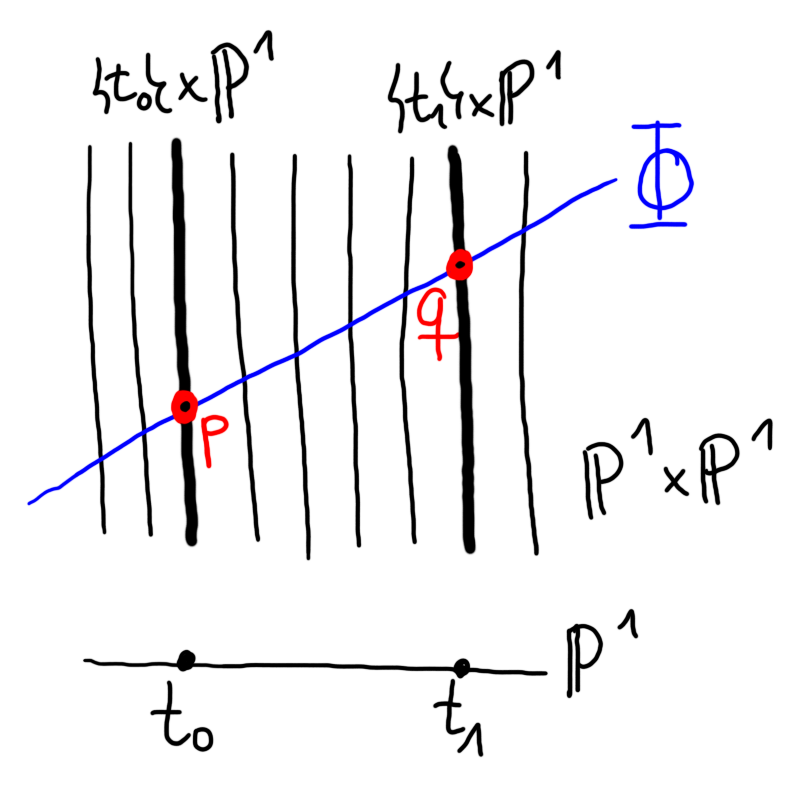
\includegraphics[scale=.2]{pictures/points}
	    \end{figure}

	\item In $\mathbb{A}^{2}$, a hyperbola is rationally equivalent to the union of two intersecting lines:
	    \begin{figure}[H]
		\centering
		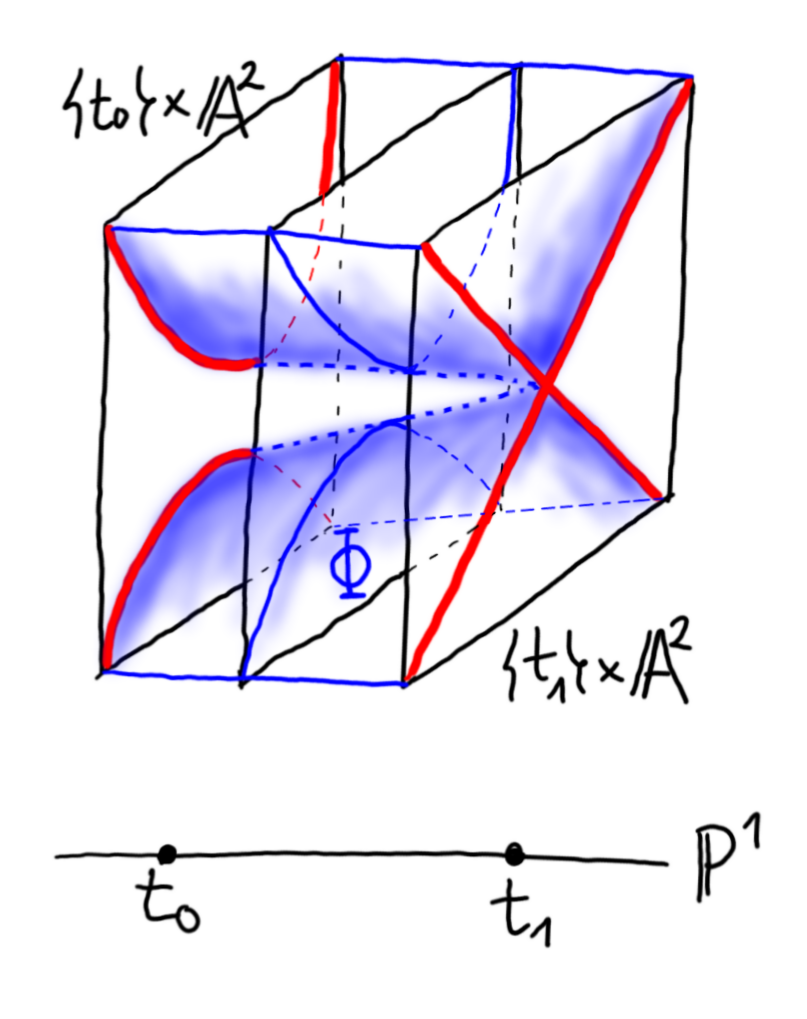
\includegraphics[scale=.2]{pictures/hyperbola}
	    \end{figure}
    \end{enumerate}
\end{exmp}

\begin{rem}\mbox{ }
    \begin{enumerate}
	\item The hypothesis that $\Phi \not\subseteq \{t\}\times X$ for any $t\in \mathbb{P}^{1}$ is essential; otherwise, any cycle on $X$ would be rationally equivalent to $0=\langle \varnothing \rangle$.
	\item \mbox{ }
	    \begin{figure}[H]
		\centering
		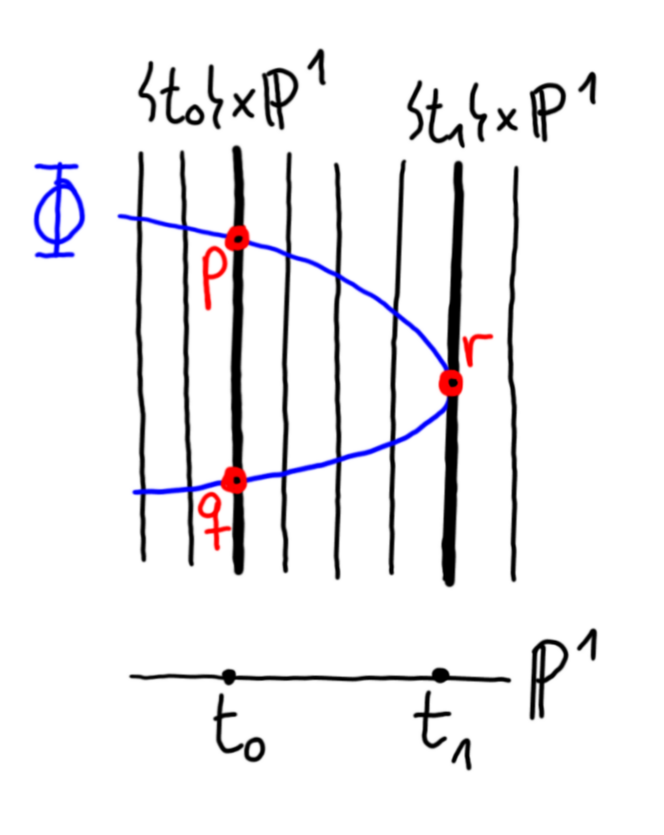
\includegraphics[scale=.2]{pictures/twotoone}
	\end{figure}
	    \[ \overset{\text{with naive intersection}}{\Rightarrow} 2[p]=[p]\Rightarrow [p]=0. \]
	    We don't want this to happen!
	    And indeed this does not happen if we consider scheme-theoretic intersections.
	    With scheme-theoretic intersections we would instead have
	    \[ [p]+[q]=2[r]\Rightarrow 2[p]=2[p], \]
	    which is okay.
    \end{enumerate}
\end{rem}

\begin{prop}
    The generators of $\operatorname{Rat}(X)$ are homogeneous with respect to the grading on $Z(X)$.
    \[ \rightsquigarrow \text{Grading on }\operatorname{CH}(X). \]
    \begin{proof}
	We need a
	\begin{lm}[{cf.~\cite[Theorem 0.2]{eh16}}]
	    If $f\colon Z\to \mathbb{P}^{1}$ is non-constant, with $Z$ a variety, then for all $p\in \mathbb{P}^{1}$ the fibre $f^{-1}(p)\subseteq Z$ has all irreducible components of codimension $1$.
	\end{lm}
	Using this, consider the map $\pi\colon \mathbb{P}^{1}\times X\to \mathbb{P}^{1}$ given by $(t,x)\mapsto t$ and restrict it to $\Phi$.
	By hypothesis, $\pi|_{\Phi}$ is non-constant, so each irreducible component of $\Phi\cap (\{t_{0}\}\times X)=\pi|_{\Phi}^{-1}(t_{0})$ has the same dimension $\dim(\Phi)-1$.

	The same holds for $\Phi\cap (\{t_{1}\}\times X)$.
    \end{proof}
\end{prop}

\subsection{Ring structure on $\operatorname{CH}^{\bullet}(X)$}

\begin{defn}[Transverse intersection]
    Two subvarieties $Z_{1},Z_{2}\subseteq X$ intersect \textit{transversally} if for every $p\in Z_{1}\cap Z_{2}$ we have that $p$ is a smooth point and that
    \[ T_{p}Z_{1}+T_{p}Z_{2}=T_{p}X. \]

    They intersect \textit{generically transversally} if this happens on a dense open subset of $Z_{1}\cap Z_{2}$.

    Two cycles $A=\sum a_{i}A_{i}$ and $B=\sum b_{j}B_{j}$ intersect generically transversally if $A_{i}$ and $B_{j}$ intersect generically transversally for all $i,j$.
\end{defn}

\begin{thmdefn}
    If $X$ is a smooth quasi-projective variety, then there is a unique ring structure on $\operatorname{CH}(X)$ satisfying:
    \begin{enumerate}[label=$(\star)$]
	\item If two subvarieties are generically transverse, then
	    \[ [A]\cdot [B]=[A\cap B]. \]
    \end{enumerate}
    Moreover, this makes $\operatorname{CH}^{\bullet}(X)$ into a graded ring.
\end{thmdefn}

The proof of theorem follows at once from the ``moving lemma'':

\begin{lm}[{\cite{ful98}}]
    Let $X$ be a smooth quasi-projective variety.
    \begin{enumerate}[label=\roman*)]
	\item For any $\alpha,\beta\in \operatorname{CH}(X)$, there are generically transverse cycles $A,B\in Z(X)$ such that $\alpha=[A]$ and $\beta=[B]$.
	\item The class $[A\cap B]$ is independent of the choice of $A$ and $B$.
    \end{enumerate}
\end{lm}

What goes wrong if $X$ is not smooth?
Both the moving lemma and the previous theorem-definition fail.

\begin{exmp}
    Let $Q\subseteq \mathbb{P}^{3}\subseteq \mathbb{P}^{4}$ be a smooth quadric, which is a surface ruled by two families of lines:
    \begin{figure}[H]
	\centering
	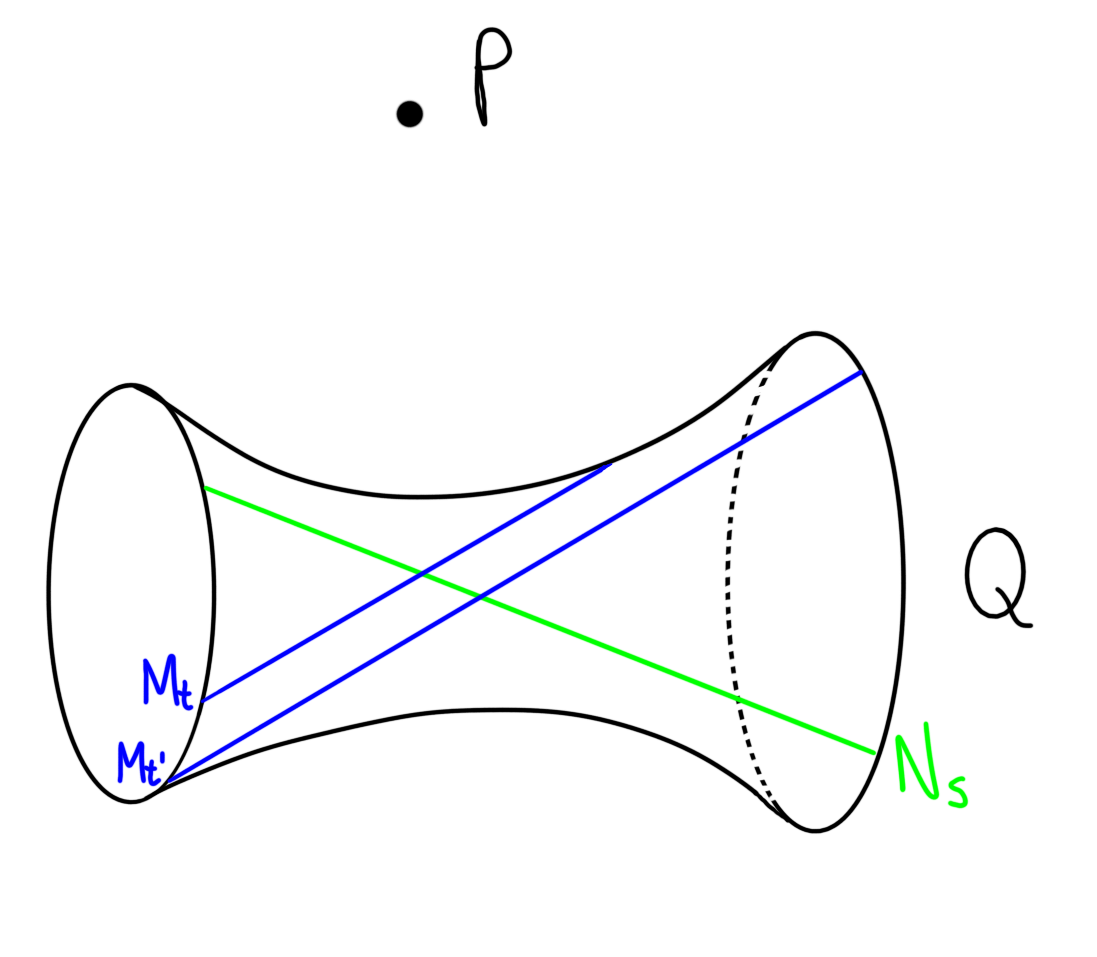
\includegraphics[scale=.2]{pictures/quadric}
    \end{figure}
    $M_{t}$ and $M_{t'}$ are in the same family, so they are disjoint.

    Let $p\in \mathbb{P}^{4}\setminus \mathbb{P}^{3}$.
    Consider $X=C(p,Q)\subseteq \mathbb{P}^{4}$, the cone with vertex $p$ and base $Q$.
    Then $X$ is ruled by two families of planes.
    \begin{figure}[H]
	\centering
	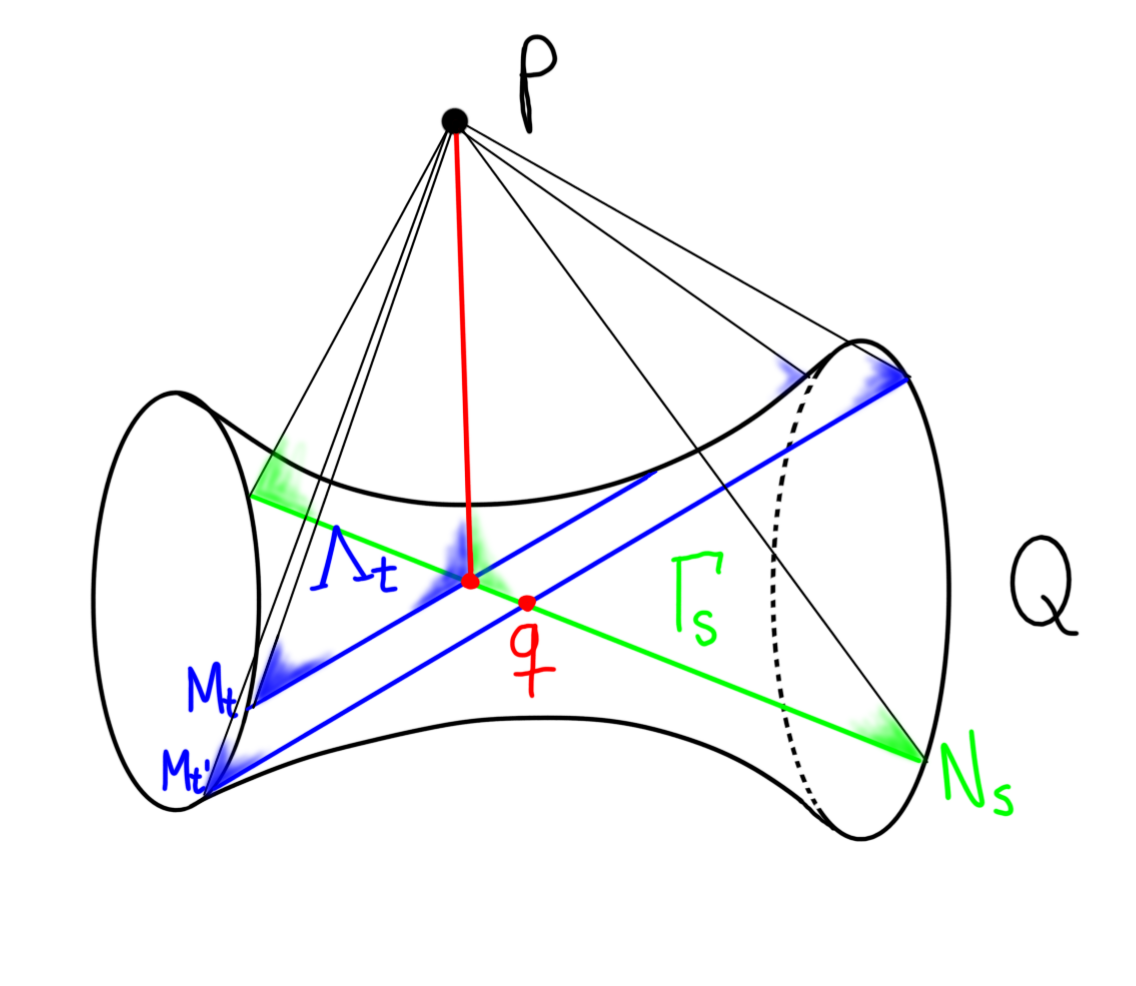
\includegraphics[scale=.2]{pictures/cone}
    \end{figure}
    In the second picture, $\Lambda_{t}=\operatorname{span}(p,M_{t})$, $\Lambda_{t'}=\operatorname{span}(p,M_{t'})$ and $\Gamma_{s}=\operatorname{span}(p,N_{s})$.
    We have $M_{t}\cap \Lambda_{t'}=\varnothing$, so they intersect transversally.
    And $N_{s}\cap \Lambda_{t'}=\{ q\}$, so they intersect transversally as well.
    We have then $[M_{t}]\cdot [\Lambda_{t'}]=0$ and $[N_{s}]\cdot [\Lambda_{t'}]=[q]$.
    But also $[M_{t}]=[N_{s}]$, because two lines in a plane are rationally equivalent, so both of them are rationally equivalent to the line $\Lambda_{t}\cap \Gamma_{s}$.
    Therefore we deduce that $[q]=0$, which cannot happen on a projective variety because of the existence of the degree map \cite[Proposition 1.21]{eh16}.
\end{exmp}

\subsection{General strategy for enumerative problems}

Prototype of enumerative problem: understand the set $\Psi$ of objects of a certain type satisfying certain conditions:

\begin{exmp}
    Lines in $\mathbb{P}^{3}$ intersecting 4 given lines $L_{1}$, $L_{2}$, $L_{3}$ and $L_{4}$.
\end{exmp}

\textbullet\underline{Step 1:} Construct a suitable (smooth, projective) parameter space $\mathcal{H}$ for the objects we are interested in, e.g.~in the case of the previous example we would look at the Grassmannian $\mathcal{H}=\mathbb{G}(1,3)$ of lines in $\mathbb{P}^{3}$.

\textbullet\underline{Step 2:} Show that for each condition imposed by our problem, the locus $Z_{i}\subseteq \mathcal{H}$ of objects satisfying that condition is closed, e.g.~in our case we would have
\[ Z_{i}=\{ L\in \mathbb{G}(1,3)\mid L\cap L_{i}\neq 0 \}, \]
so that $\Psi=\cap_{i=1}^{4}Z_{i}\subseteq \mathcal{H}$ is closed.

\textbullet\underline{Step 3:} Describe $\operatorname{CH}^{\bullet}(\mathcal{H})$ and $[Z_{i}]\in \operatorname{CH}^{\bullet}(\mathcal{H})$, which in the case of our example will be done in future talks of this seminar.

\textbullet\underline{Step 4:} Calculate the product $\prod_{i}[Z_{i}]$.
Then $[\Psi]=[\cap_{i}Z_{i}]=\prod_{i}[Z_{i}]$, assuming that the intersections are generically transverse.
So if things work out well and we are a bit careful, we can obtain the answer as the degree \cite[Propostion 1.21]{eh16} of some zero cycle $[\Psi]$ in our (smooth, projective) parameter space $\mathcal{H}$.

\section{Jin Li: Basic computational tools (13.01.2021)}

\subsection{Recollections}

An \textit{algebraic set} is a closed subset in $\mathbb{A}^{n}$ (or $\mathbb{P}^{n}$) in the Zariski topology.
A \textit{scheme} is the datum of an algebraic set together with the ideal defining it.

\begin{rem}
    A scheme can be non-reduced and non-irreducible, e.g.~$X=V(xy^{2})\subseteq \mathbb{A}^{2}$.
    \begin{figure}[H]
	\centering
	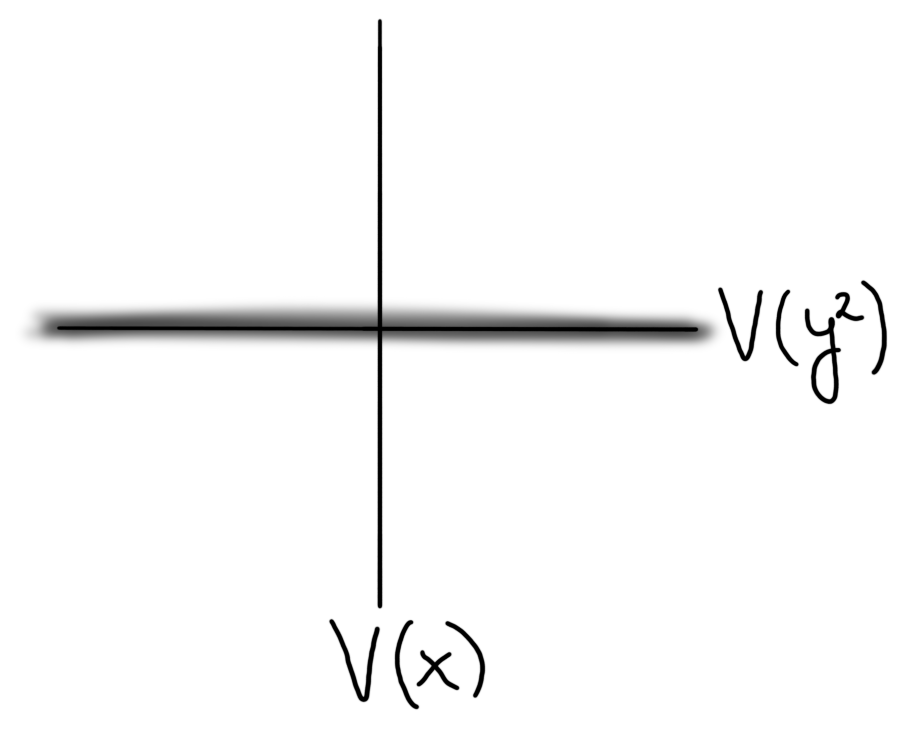
\includegraphics[scale=.75]{pictures/schemeaxes}
    \end{figure}

    Reduced means that every irreducible component has multiplicity one.
\end{rem}

An \textit{algebraic variety} is a reduced an irreducible scheme in $\mathbb{A}^{n}$ (\textit{affine variety}) or in $\mathbb{P}^{n}$ (\textit{projective variety}).

Let $X$ be an algebraic variety.
The \textit{group of cycles} on $X$, denoted $Z(X)$, is a free abelian group generated by subvarieties of $X$.
$Z(X)=\oplus_{k\in \mathbb{N}}Z_{k}(X)$ is graded by dimension, and the elements in $Z_{k}(X)$ are called $k$-cycles for each $k\in \mathbb{N}$.
To any closed subscheme $Y\subseteq X$ we associate a cycle
\[ \langle Y\rangle :=\sum_{i=1}^{s}m_{i}Y_{i}, \]
for example $\langle V(xy^{2})\rangle = V(x)+2V(y)$.

We define $\operatorname{Rat}(X)\subseteq Z(X)$ as the subgroup generated by expressions of the form
\begin{equation}\label{eqn:2.1}
    \langle \Phi\cap (\{t_{0}\}\times X)\rangle - \langle \Phi\cap (\{t_{1}\}\times X)\rangle,
\end{equation}
where $t_{0},t_{1}\in \mathbb{P}^{1}$ and $\Phi\subseteq \mathbb{P}^{1}\times X$ is a subvariety not contained in any fibre $\{ t\}\times X$.

Two cycles $A_{0},A_{1}\in Z(X)$ are called \textit{rationally equivalent} if $A_{1}-A_{0}\in \operatorname{Rat}(X)$.

In \Cref{eqn:2.1} we take the scheme theoretic intersection, which means that we need to consider the multiplicities, e.g.~the picture
\begin{figure}[H]
    \centering
    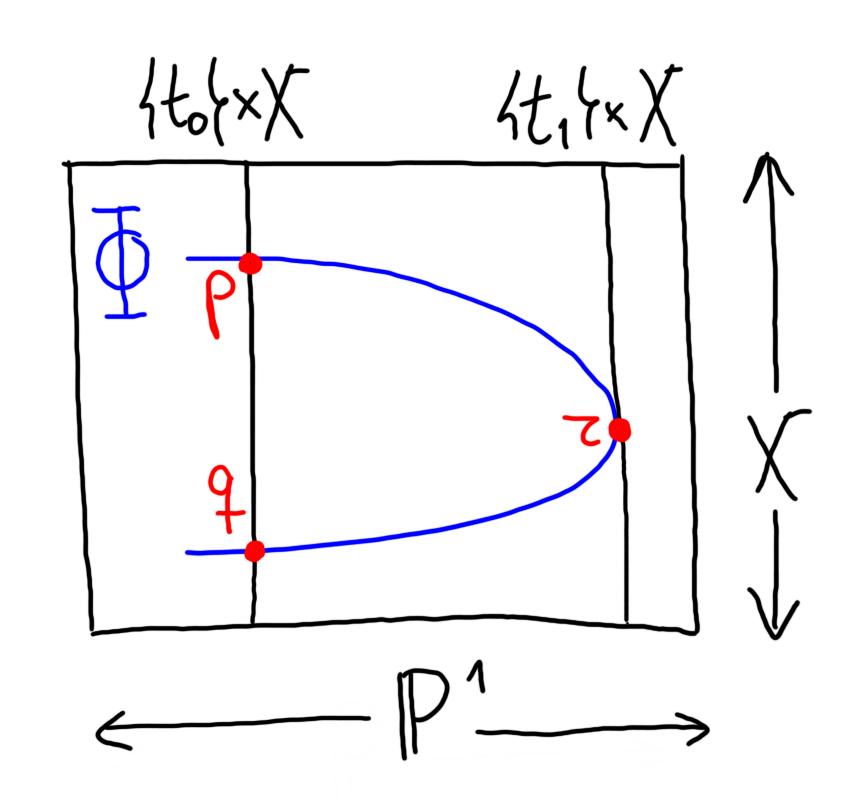
\includegraphics[scale=.75]{pictures/equivalence}
\end{figure}

implies that $p+q\sim 2\tau$ and not $p+q\sim \tau$.

$\Phi$ not being contained in any fibre is necessary, otherwise we would have $A\sim 0=\langle \varnothing \rangle$ for all $A\in Z(X)$.

We define the \textit{Chow group} of $X$, denoted $A(X)$ or $\operatorname{CH}(X)$, as
\[ A(X):=Z(X)/\operatorname{Rat}(X). \]

For a cycle $Y\in Z(X)$, we denote by $[Y]\in A(Y)$ its equivalence class in $A(X)$.
When $Y\subseteq X$ is a subscheme, we also denote simply by $[Y]$ the equivalence clas in $A(X)$ of the cycle $\langle Y\rangle$ associated to $Y$.
For example,
\[ [V(xy^{2})]=[V(x)]+2[V(y)]. \]

The Chow group is graded by dimension $A(X)=\oplus_{k=0}^{\dim(X)}A_{k}(X)$.
We have seen the following

\begin{thmdefn}
    If $X$ is a smooth quasi-projective variety, then there is a unique ring structure on $A(X)$ satisfying:
    \begin{enumerate}[label=$(\star)$]
	\item If two subvarieties are generically transverse, then
	    \begin{equation}\label{eqn:2.2}
		[A]\cdot [B]=[A\cap B].
	    \end{equation}
    \end{enumerate}
\end{thmdefn}

This structure makes $A(X)$ a graded ring, graded by codimension
\[ A(X)=\oplus_{c=0}^{\dim(X)}A^{c}(X), \quad c=\dim(X)-k. \]
We call it the \textit{Chow ring} of $X$.

\begin{rem}
    \Cref{eqn:2.2} holds more generally as long as
    \[ \operatorname{codim}(A\cap B)=\operatorname{codim}(A)+\operatorname{codim}(B). \]
\end{rem}

\begin{exmp}
    In $\mathbb{P}^{3}$ we have:
    \begin{figure}[H]
	\centering
	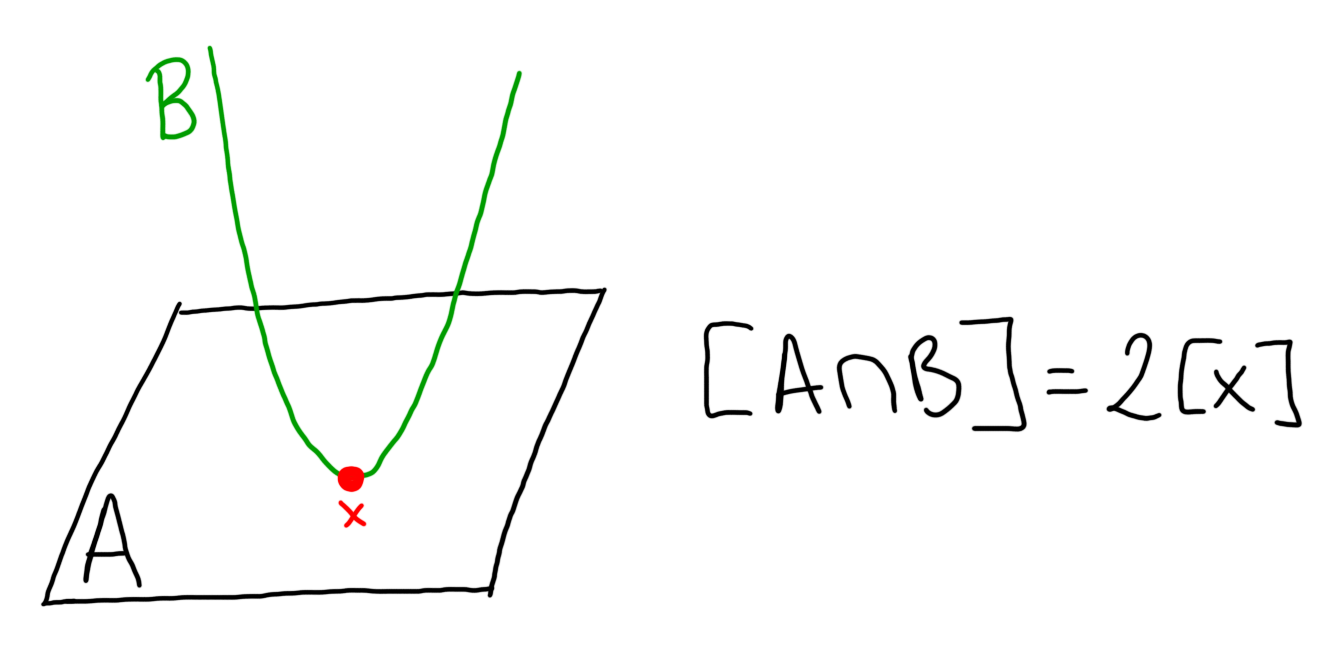
\includegraphics[scale=.75]{pictures/planeandparabola}
    \end{figure}

    But the moving lemma implies that we can move the curve within its rational equivalence class:
    \begin{figure}[H]
	\centering
	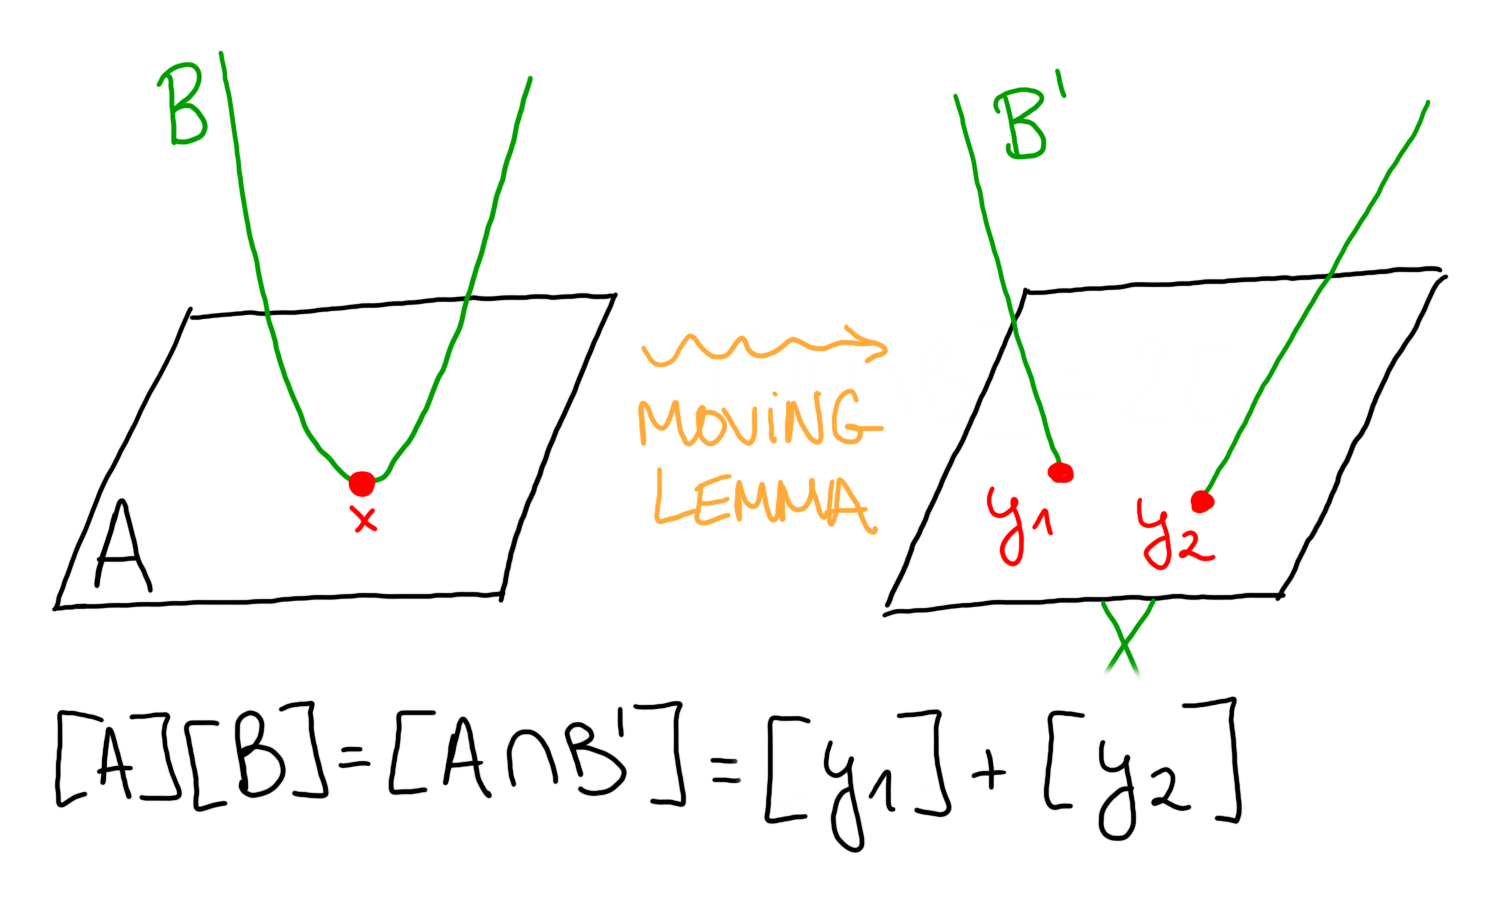
\includegraphics[scale=.75]{pictures/parabolatolines}
    \end{figure}
\end{exmp}

\subsection{The Chow ring of affine space}

\begin{prop}
    If $X$ is a variety of dimension $n$, then its fundamental class $[X]\in A(X)$ is always non-zero.
    \begin{proof}
	If $[X]=0$, then $[X]$ could be written as a $\mathbb{Z}$-linear combination of expressions as in \Cref{eqn:2.1}.
	We claim that only when $\Phi=\mathbb{P}^{1}\times X$ can $X$ appear as the result of an expression of the form $\Phi\cap (\{t\}\times X)$, but in this case we would just have $X\sim X$.

	Suppose then that $\Phi\subsetneq \mathbb{P}^{1}\times X$.
	By definition of dimension and irreducibility of $\Phi$ and of $\mathbb{P}^{1}\times X$, we must have
	\[ \dim(\Phi)\leq n=\dim(X). \]
	On the other hand, since we are assuming that $X$ appears as the result of an expression $\langle \Phi\cap (\{ t\}\times X)\rangle$, we must have
	\[ \{t\}\times X\subseteq \Phi, \]
	thus $\{t\}\times X=\Phi$, because both are irreducible, $\{t\}\times X$ has dimension $n$ and $\Phi$ has dimension at most $n$.
	But this contradicts then the assumption that $\Phi$ is not contained in any fibre $\{t\}\times X$, hence the previous situation cannot occur.
    \end{proof}
\end{prop}

So from this proposition we deduce that $A^{0}(X)=\mathbb{Z}\cdot [X]$.

\begin{prop}
    For affine space $\mathbb{A}^{n}$ we have
    \[ A(\mathbb{A}^{n})=\mathbb{Z}\cdot [\mathbb{A}^{n}]. \]
    \begin{proof}
	We have already seen that $A^{0}(\mathbb{A}^{n})=\mathbb{Z}\cdot [\mathbb{A}^{n}]$, so it suffices to show that all other subvarieties $Y\subsetneq \mathbb{A}^{n}$ are rationally equivalent to $0=\langle \varnothing\rangle$.

	Given such $Y$, we want to construct a $\Phi$ interpolating between $Y$ and $\varnothing$.
	Choose coordinates $z=(z_{1},ldots,z_{n})$ such that $0\not\in Y$ and let $Y=V(I)$ for some ideal $I$.
	We define
	\[ W^{\circ}:=\{(t,tz)\in (\mathbb{A}^{1}\setminus \{0\})\times \mathbb{A}^{n}\mid z\in Y\}=V(\{f(z/t)\mid f\in I\}). \]
	The fibre of $W^{\circ}$ over $t$ is $tY$.
	Let $W:=\overline{W^{\circ}}\subseteq \mathbb{P}^{1}\times \mathbb{A}^{n}$ be the closure.
	The claim is that $\Phi=W$ is the variety interpolating between $Y$ and $\varnothing$.
	The fibre of $W$ over $t=1$ is then just $Y$.
	So our goal is to show that there is some other fibre which is empty, and we will see that this is the fibre over $t=\infty\in \mathbb{P}^{1}$.
	\begin{figure}[H]
	    \centering
	    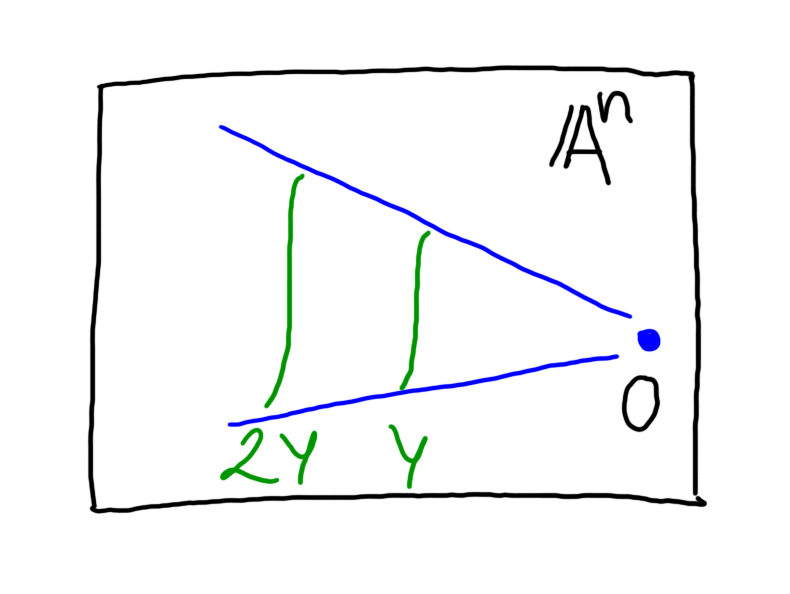
\includegraphics[scale=.9]{pictures/scaling}
	\end{figure}

	Since $0\not\in Y$, we can find some $g\in I$ which has non-zero constant term $c$.
	Define then
	\[ G(t,z):=g(z/t) \]
	on $(\mathbb{A}^{1}\setminus \{0\})\times \mathbb{A}^{n}$.
	For $t=\infty$ we get $G(\infty,z)=g(0)=c$ for all $z\in \mathbb{A}^{n}$, so $G$ extends to a regular function on $(\mathbb{P}^{1}\setminus \{0\})\times \mathbb{A}^{n}$.
	We have $W^{\circ}\subseteq V(G)$, so $W\subseteq V(G)$ as well.
	Since $V(G)\cap (\{\infty\}\times \mathbb{A}^{n})=V(G(\infty,z))=V(c)=\varnothing$, we also have $W\cap (\{\infty\}\times \mathbb{A}^{n})=\varnothing$, therefore
	\[ Y\sim 0. \]
    \end{proof}
\end{prop}

\subsection{Functoriality \cite[\S 1.2.6]{eh16}}

Let $X$ and $Y$ be schemes, $f\colon Y\to X$ be a proper map (``closed map with compact fibres''), e.g.~any map between projective varieties.
If $A\subseteq Y$ is a subvariety, then $f(A)\subseteq X$ is a subvariety.
Therefore, one may be tempted to define $f_{*}([A]):=[f(A)]$.
But this naive definition caues some problems.
The key problem are the multiplicities:
\begin{figure}[H]
    \centering
    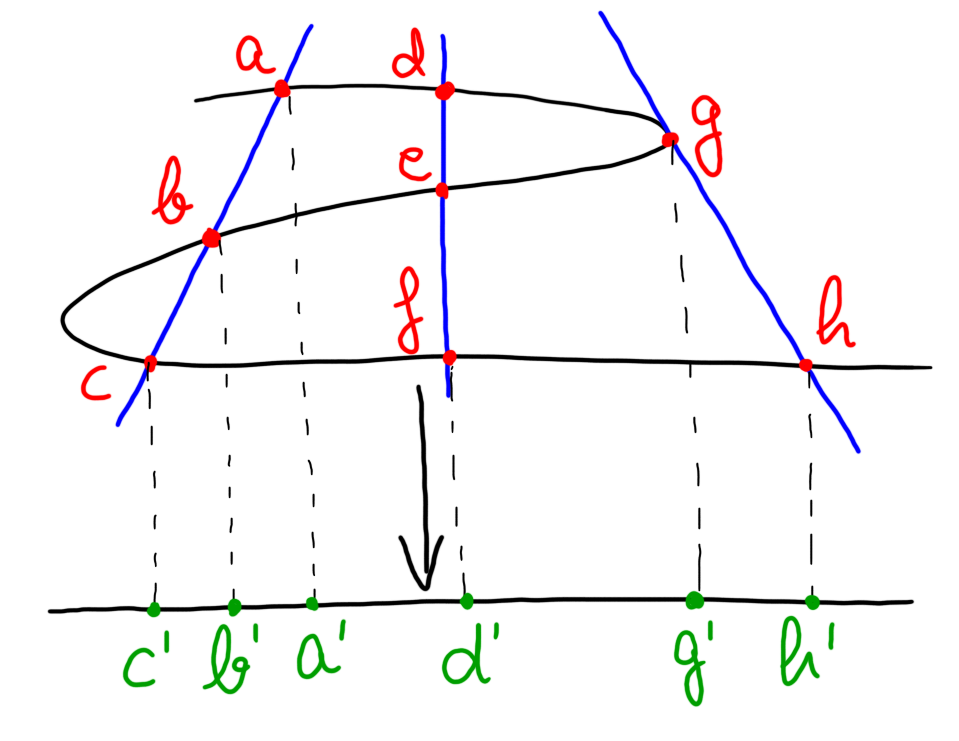
\includegraphics[scale=.9]{pictures/pushforward}
\end{figure}

With the naive definition we would have $a'+b'+c'\sim d'\sim g'+h'$, which is a contradiction because all points are rationally equivalent in $\mathbb{P}^{1}$ and as we will soon see they are non-zero.
With the correct definition we would instead have
\[ a'+b'+c'\sim 3d'\sim 2g'+h'. \]

\begin{defn}
    If $\dim(f(A))<\dim(A)$, then we set $f_{*}([A])=0$.
    And if $\dim(f(A))=\dim(A)$, then we set $f_{*}([A])=n[f(A)]$, where $n=[\mathbb{C}(A):\mathbb{C}(f(A))]$ is the degree of $f|_{A}$.
    We extend $f_{*}$ to all cycles by linearity, that is,
    \[ f_{*}(\sum m_{i}[A_{i}])=\sum m_{i}f_{*}([A_{i}]). \]
\end{defn}

\begin{thm}[{\cite[\S 1.4]{ful98}}]
    If $f\colon Y\to X$ is proper, then $f_{*}\colon Z(Y)\to Z(X)$ induces a group homomorphism $f_{*}\colon A_{k}(Y)\to A_{k}(X)$ for all $k\in \mathbb{N}$.
\end{thm}

As a particular case we obtain the existence of the degree map, which was already used in an example during the previous talk:

\begin{prop}
    If $X$ is proper, that is, if the structure map to a point $X\to \operatorname{Spec}{\mathbb{C}}$ is proper, then there exists a unique group homomorphism $\deg\colon A(X)\to \mathbb{Z}$, called the \textit{degree map}, taking every closed point $p\in X$ to $1\in\mathbb{Z}$ and vanishing on the classes of cycles of dimension greater than $0$.
\end{prop}

If $A$ is a $k$-dimensional subvariety of a smooth projective $n$-dimensional variety $X$ and $B$ is an $(n-k)$-dimensional subvariety of $X$ such that $A\cap B$ is finite and non-empty, then the existence of the group homomorphism
\begin{align*}
    A_{k}(X) & \longrightarrow \mathbb{Z} \\
    [A] & \longmapsto \deg([A]\cdot [B])>0
\end{align*}
guarantees that $[A]\neq 0$.

Let now $f\colon Y\to X$ be a flat morphism between schemes.
We will not define flatness, but important examples are open inclusions and morphisms between smooth varieties with all fibres of the same dimension \cite[Corollary 14.128]{gw10}.
Then
\begin{align*}
    f^{*}\colon A(X) & \longrightarrow A(Y) \\
    \langle A\rangle & \longmapsto \langle f^{-1}(A)\rangle
\end{align*}
prevserves rational equivalence and induces a group homomorphism between the Chow rings preserving the grading by codimension.

\subsection{Mayer--Vietoris and excision \cite[\S 1.3.4]{eh16}}

\begin{prop}
    Let $X$ be a scheme.
    \begin{enumerate}[label=(\alph*)]
	\item \textit{(Mayer--Vietoris)} If $X_{1},X_{2}$ are closed subschemes of $X$, then there is a right exact sequence
	    \[ A(X_{1}\cap X_{2})\to A(X_{1})\oplus A(X_{2})\to A(X_{1}\cup X_{2})\to 0. \]
	    The map on the left is given by $[W]\mapsto ([W],-[W])$, whereas the one on the right is given by $([W_{1}],[W_{2}])\mapsto [W_{1}]+[W_{2}]$.
	\item \textit{(Excision)} If $Y\subseteq X$ is a closed subscheme and $U=X\setminus Y$, then there is a right exact sequence
	    \[ A(Y)\mapsto A(X)\mapsto A(U)\mapsto 0. \]
	    The map on the left is proper pushforward along the closed immersion $Y\subseteq X$, whereas the map on the right is the flat pullback along the open immersion $U\subseteq X$.
	    If $X$ is smooth, then $A(X)\to A(U)$ is moreover a ring homomorphism.
    \end{enumerate}
\end{prop}

\begin{cor}
    If $U\subseteq \mathbb{A}^{n}$ is a non-empty open subset, then
    \[ A(U)=\mathbb{Z}\cdot [U]. \]
    \begin{proof}
	If we define $Y:=\mathbb{A}^{n}\setminus U$, then we have the excision right exact sequence
	\[ A(Y)\to A(\mathbb{A}^{n})\to A(U)\to 0. \]
	If $W\subseteq Y$ is a subvariety, then $[W]=0$ seen as a class in $A(\mathbb{A}^{n})$, as we saw earlier.
	Therefore the map on the left is the zero map and the result follows.
    \end{proof}
\end{cor}

\subsection{Stratifications \cite[\S 1.3.5]{eh16}}

\begin{defn}
    Let $X$ be a scheme.
    We say that $X$ is \textit{stratified} by a finite collection $\{ U_{i}\}_{i=1}^{m}$ of irreducible, locally closed subschemes $U_{i}$ if the following hold:
    \begin{enumerate}[label=\roman*)]
	\item $X=\sqcup_{i=1}^{m} U_{i}$ is a disjoint union; and
	\item each closure $\overline{U_{i}}$ is a union of some $U_{j}$'s.
    \end{enumerate}
\end{defn}

Condition $ii)$ can be rephrased by saying that
\[ \overline{U_{i}}\cap U_{j}\neq \varnothing \Rightarrow U_{j}\subseteq \overline{U_{i}}. \]

The $U_{i}$ are called \textit{strata} and the $Y_{i}:=\overline{U_{i}}$ are called \textit{closed strata}.
We can recover $U_{i}$ from $Y_{i}$ by the formula
\[ U_{i}=Y_{i}\setminus \left(\bigcup_{Y_{j}\subsetneq Y_{i}} Y_{j}\right). \]

We say that a stratification is \textit{affine} if for each $i$ there exists an $l\in \mathbb{N}$ such that $U_{i}\cong \mathbb{A}^{l}$.
We say that it is \textit{quasi-affine} if for each $i$ there exists an $l\in \mathbb{N}$ such that $U_{i}$ is isomorphic to an open subset in $\mathbb{A}^{l}$.

\begin{exmp}
    Projective $n$-space admits an affine stratification with closed strata given by
    \[ \mathbb{P}^{0}\subseteq \mathbb{P}^{1}\subseteq \ldots \subseteq \mathbb{P}^{n}. \]
    It is affine because $\mathbb{P}^{i}\setminus \mathbb{P}^{i-1}\cong \mathbb{A}^{i}$.
\end{exmp}

\begin{prop}[{\cite[Proposition 1.17]{eh16}}]
    If a scheme $X$ has a quasi-affine stratification, then $A(X)$ is generated by the classes of the closed strata.
\end{prop}

\begin{rem}
    It can happen that the clases of the strata in a quasi-affine stratification become zero in the Chow ring.
    For instance, consider $\mathbb{A}^{n}$ with $n>0$ and the stratification
    \[ \mathbb{A}^{n}=\{0\}\cup (\mathbb{A}^{n}\setminus \{ 0 \}), \]
    with $U_{0}=\{0\}$ and $U_{1}=\mathbb{A}^{n}\setminus \{0\}$.
    Then $Y_{0}=\{ 0\}$ has $[Y_{0}]=0\in A(\mathbb{A}^{n})$, as we saw earlier in the talk.
\end{rem}

But in the case of affine stratifications we have the following:

\begin{thm}[Totaro, 2014]
    The classes of the closed strata in an affine stratification of a scheme $X$ form a basis of $A(X)$.
\end{thm}

\section{Vincent Gajda: Grassmannians and Schubert varieties (20.01.21)}

\textbf{Goal:} introduce Grassmannians (working always over $\mathbb{C}$ or over an algebraically closed field of characteristic $0$).

\subsection{Recall stratifications}

We say that $X$ is \textit{stratified} by a finite family $\{U_{i}\}_{i\in I}$ of locally closed subvarieties if
\[ X=\bigsqcup_{i\in I}U_{i}, \text{ and } \overline{U_{i}}=\bigsqcup_{j\in J}U_{j} \text{ for some }J\subseteq I. \]

A stratification is called \textit{affine} if each $U_{i}$ is isomorphic to an affine space $\mathbb{A}^{n_{i}}$, and \textit{quasi-affine} if each $U_{i}$ is isomorphic to a non-empty open subset inside an affine space $\mathbb{A}^{n_{i}}$.

\begin{prop}
    If $X$ is quasi-affinely stratified, then $A(X)$ is generated as a group by the classes of the closed strata, i.e.~the classes of the Zariski closures of the $U_{i}$.
    \begin{proof}
	We argue by induction on the number of strata.
	Let $U_{0}$ be a minimal stratum.
	By definition of stratification, it has to be a closed subset of $X$, and the open subset $X\setminus U_{0}$ admits a quasi-affine stratification with one less stratum than the original quasi-affine stratification of $X$.
	We have seen in the last talk that $A(U_{0})=\mathbb{Z}\cdot [U_{0}]$, because $U_{0}$ is isomorphic to a non-empty open subset inside some affine space.
	The result follows then from the induction hypothesis and the excision exact sequence
	\[ \mathbb{Z}\cdot [U_{0}]\to A(X)\to A(X\setminus U_{0})\to 0. \]
    \end{proof}
\end{prop}

\subsection{Chow ring of $\mathbb{P}^{n}$}

\begin{defn}
    Let $X\subseteq \mathbb{P}^{n}$ be a projective variety of dimension $k$.
    Then we define its \textit{degree}, denoted $\deg(X)$, as the number of points in the intersection of $X$ with a generically transverse $(n-k)$-plane.
    If $X\subseteq \mathbb{P}^{n}$ is only a subscheme, then we add the degrees of its irreducible components with multiplicities.
\end{defn}

\begin{rem}
    One can use Hilbert polynomials to define the degree of a projective variety and make sure that it is indeed a well-defined number.
\end{rem}

\begin{thm}[Kleiman]
    Suppose $G$ is an algebraic group ($\operatorname{GL}_{n}$ suffices for our purposes) that acts transversally on an algebraic variety $X$.
    Let $A\subseteq X$ be a subvariety.
    \begin{enumerate}
	\item Let $B\subseteq X$ be another subvariety.
	    Then there exists a dense open subset $G_{0}\subseteq G$ such that for all $g\in G_{0}$, $g\cdot A$ intersects $B$ generically transversally.
	\item If $G$ is affine (again, we may just think of $\operatorname{GL}_{n}$), then $[A]=[g\cdot A]$ for all $g\in G$.
    \end{enumerate}
    \begin{proof}
	See \cite[Theorem 1.7]{eh16}.
	The assumptions on the base field are important here!
    \end{proof}
\end{thm}

\begin{exmp}
    $\operatorname{GL}_{n+1}$ acts transitively on $\mathbb{P}^{n}$, so all $k$-planes in $\mathbb{P}^{n}$ define the same class in the Chow ring.
\end{exmp}

\begin{prop}
    We have
    \[ A(\mathbb{P}^{n})=\mathbb{Z}[\zeta]/(\zeta^{n+1}), \]
    where $\zeta\in A^{1}(\mathbb{P}^{n})$ is the class of a hyperplane.
    Moreover, if $X\subseteq \mathbb{P}^{n}$ is a subvariety of codimension $k$ and degree $d$, then $[X]=d\zeta^{k}$.
    \begin{proof}
	Let $\{p\}\subseteq \mathbb{P}^{1}\subseteq \ldots \subseteq \mathbb{P}^{n}$ be a complete flag.
	These are the closed strata of an affine stratification, so we know that the classes of $\mathbb{P}^{i}$ generates $A^{n-i}(\mathbb{P}^{n})$ for each $i\in \{0,\ldots,n\}$.
	By Kleiman's theorem we deduce moreover that the class of any $i$-plane generates $A^{n-i}(\mathbb{P}^{n})$.
	We saw in the previous talk that there exists a well-defined surjective degree map
	\begin{align*}
	    \deg\colon A^{n}(\mathbb{P}^{n}) &\longrightarrow \mathbb{Z} \\
	    [p] & \longmapsto 1
	\end{align*}
	We have just seen that $A^{n}(\mathbb{P}^{n})$ is generated by a signle point, so in order for $\deg$ to be surjective we need to have $A^{n}(\mathbb{P}^{n})=\mathbb{Z}\cdot [p]$.

	Let now $M$ be a $k$-plane and take a generically transverse generator of $A^{k}(\mathbb{P}^{n})$.
	The intersection contains exactly $1$ point, so
	\[ [M]\cap \colon A^{k}(\mathbb{P}^{n})\to A^{n}(\mathbb{P}^{n})\cong \mathbb{Z} \]
	is also surjective.
	By the same argument as before we must have $A^{k}(\mathbb{P}^{n})\cong \mathbb{Z}$.

	Now for the ring structure, we know that an $(n-k)$-plane $L$ is the transverse interecction of $k$ hyperplanes, so we have
	\[ [L]=\zeta^{k}, \]
	where $\zeta$ is the class of any hyperplane.
	This implies that the ring structure is as claimed.

	Finally, if $X\subseteq \mathbb{P}^{n}$ is a subvariety of codimension $k$ and degree $d$, then the assumption on the codimension implies that $[X]\in A^{k}(\mathbb{P}^{n})=\mathbb{Z}\cdot \zeta^{k}$, so we may write $[X]=m\zeta^{k}$.
	The assumption on the degree implies then that
	\[ d=\deg([X]\cdot \zeta^{n-k})=\deg(m\zeta^{k}\zeta^{n-k})=m, \]
	as we wanted to show.
    \end{proof}
\end{prop}

\begin{cor}[B\'{e}zout]
    If $X_{1},\ldots,X_{k}\subseteq \mathbb{P}^{n}$ are subvarieties of codimensions $c_{1},\ldots,c_{k}$ respectively, with $\sum c_{i}\leq n$ and intersecting generically transversely, then
    \[ \deg(X_{1}\cap \ldots \cap X_{k})=\prod \deg(X_{i}). \]
    In particular, if $X,Y\subseteq \mathbb{P}^{n}$ have complementary dimensions and intersect generically transversely, then
    \[ |X\cap Y|=\deg(X)\deg(Y). \]
    \begin{proof}
	By the previous proposition we can write
	\[ [X_{i}]=\deg(X_{i})\zeta^{c_{i}} \]
	for each $i\in \{1,\ldots,k\}$.
	On the ohter hand,
	\[ [X_{1}\cap \ldots\cap X_{k}]=\deg(X_{1}\cap\ldots\cap X_{k})\zeta^{\sum c_{i}}. \]
	But
	\[ [X_{1}\cap \ldots \cap X_{k}]=[X_{1}]\cdots [X_{k}]=\left(\prod \deg(X_{i})\right)\zeta^{\sum c_{i}}, \]
	hence the desired equality.
    \end{proof}
\end{cor}

\subsection{Grassmannians}

Let $V$ be an $n$-dimensional vector space over $\mathbb{C}$ and let $1\leq k\leq n$.
We want to consider the \textit{Grassmannian} of $k$-planes in $V$:

\[ G:=G(k,V):=\left\{ \begin{array}{c}
    k\text{-dimensional} \\
    \text{subspaces in }V
    \end{array}\right\}
    =\left\{ \begin{array}{c}
    (k-1)\text{-dimensional} \\
    \text{subspaces in }\mathbb{P}(V)
    \end{array} \right\}
\]
We would write $\mathbb{G}(k-1,V)$ instead to mean the right-hand side interpretation of $(k-1)$-dimensional subspaces in $\mathbb{P}(V)$.
	
We have described the Grassmannian as a set, but we want to endow it with a structure of projective variety.
We consider for this the \textit{Plücker embedding}:

\begin{align*}
    G & \longrightarrow \mathbb{P}(\wedge^{k}V)\cong \mathbb{P}^{\binom{n}{k}-1} \\
    \Lambda=\langle w_{1},\ldots,w_{n}\rangle & \longmapsto [w_{1}\wedge \ldots \wedge w_{k}]
\end{align*}

This map is well-defined, because if we had chosen a different basis for $\Lambda$, then the result would have only differed by multiplication with the (non-zero) determinant of the base-change matrix.
And it is injective, because a vector $v\in V$ is in $\Lambda$ if and only if $v\wedge (w_{1}\wedge\ldots \wedge w_{k})=0$, so we can recover $\Lambda$ from $[w_{1}\wedge\ldots\wedge w_{k}]$.

If we choose a basis $\{ e_{1},\ldots,e_{n}\}$ of $V$, then we may identify $V$ with $\mathbb{C}^{n}$ and represent $\Lambda$ as the row space of a $k\times n$ matrix

\[ A=\begin{pmatrix}
    a_{1,1} & \cdots & a_{1,n} \\
    \vdots & & \vdots \\
    a_{k,1} & \cdots & a_{k,n}
\end{pmatrix} \]

in which the rows are the $w_{1},\ldots,w_{k}$.
We may then write
\[ w_{1}\wedge \ldots \wedge w_{k}=\sum_{1\leq i_{1}<\ldots<i_{k}\leq n} p_{i_{1},\ldots,i_{k}}e_{i_{1}}\wedge \ldots e_{i_{k}}, \]
and these coefficients $p_{i_{1},\ldots,i_{k}}$ are called the \textit{Plücker coordinates} of $\Lambda$ with respect to the basis $\{ e_{1},\ldots,e_{n}\}$.
They do not depend on the chosen basis for $\Lambda$, because each $p_{i_{1},\ldots,i_{k}}$ is given by the corresponding minor of $A$, and changing the basis of $\Lambda$ corresponds to multiplying $A$ on the left by an invertible $k\times k$ matrix.
Therefore they are well-defined as coordinates in $\mathbb{P}^{\binom{n}{k}-1}$.

Next we want to argue that the Plücker embedding $\varphi\colon G\hookrightarrow \mathbb{P}^{\binom{n}{k}-1}$ makes $G$ an algebraic variety.
Let us call a point of the form $[w_{1}\wedge\ldots \wedge w_{k}]\in \mathbb{P}(\wedge^{k}V)$ a \textit{pure wedge product}.
Then $\varphi(G)$ consists precisely of the equivalence classes of pure wedge products, so we need to find homogeneous polynomial equations describing the set of such equivalence classes.
If $\eta\in \wedge^{k}V$ and $v\in V\setminus \{0\}$, then $v\wedge \eta=0$ if and only if $\eta=v\wedge \eta'$ for some $\eta'\in \wedge^{k-1}V$.
By induction we deduce that $\eta$ is a pure wedge product if and only if
\[ \dim\left(V\xrightarrow{(-)\wedge\eta}\wedge^{k+1}V\right)\geq k, \]
therefore
\[ \varphi(G)=\left\{ [\eta]\in \mathbb{P}(\wedge^{k}V) \middle| \operatorname{rank}\left(V\xrightarrow{(-)\wedge \eta} \wedge^{k+1}V\right) \leq n-k \right\}. \]
This subspace of $\mathbb{P}(\wedge^{k}V)$ is the zero locus of the $(n-k+1)$-minors of a matrix representing the linear map $(-)\wedge \eta$, which are homogeneous polynomials.
Hence $\varphi(G)$ is an algebraic subset in $\mathbb{P}^{\binom{n}{k}-1}$.
To check that $G$ is also a variety, i.e.~to check that it is irreducible, note that its ideal is the kernel of the ring homomorphism
\[ \mathbb{C}[\{p_{i_{1},\ldots,i_{k}}\}_{1\leq i_{1}<\ldots i_{k}\leq n}] \longrightarrow \mathbb{C}[\{ x_{ij}\}_{1\leq i\leq n,1\leq j\leq k}] \]
which corresponds to ``writing out the Pl\"{u}cker coordinates'' in terms of the coefficients of the matrix.
The ring on the right is an integral domain, so the kernel of this morphism is a prime ideal and $G$ is an algebraic variety.
In the following we often identify $G$ with $\varphi(G)$ as sets already.

As in the particular case of projective spaces, Grassmannians admit a \textit{standard affine open cover} constructed as follows.
Fix $\Gamma \subseteq V$ of dimension $(n-k)$, say $\Gamma=\langle e_{1},\ldots,e_{n-k}\rangle$.
We may extend this basis of $\Gamma$ to a basis $e_{1},\ldots,e_{n}$ of $V$, and we let $\eta:=e_{1}\wedge\ldots \wedge e_{n-k}$.
Define
\[ U_{\Gamma}:=\{ \Lambda\in G\mid \Lambda\cap \Gamma = 0\}. \]
The complement of $U_{\Gamma}$ is the set of $[\omega]\in G$ such that $\omega\wedge \eta=0$, which can be characterized as the hyperplane section where the $(e_{1},\ldots,e_{n})$-Pl\"{u}cker coordinate $p_{n-k+1,\ldots,n}$ is equal to zero.
Hence $U_{\Gamma}$ is open, and as we vary the subspace $\Gamma$ we obtain an open cover of $G$.
From this open cover we deduce that $\dim{G}=k(n-k)$ and that $G$ is smooth, because we have the following

\begin{lm}
    $U_{\Gamma}\cong \mathbb{A}^{k(n-k)}$.
    \begin{proof}
	Consider a basis $(e_{1},\ldots,e_{n})$ of $V$ such that $\Gamma=\langle e_{k+1},\ldots,e_{n}\rangle$.
	Then we have
	\[ U_{\Gamma}=\{ \Lambda\in G\mid p_{1,\ldots,k}(\Lambda)\neq 0\}. \]
	We regard $\mathbb{A}^{k(n-k)}$ as the space of $k\times (n-k)$-matrices, and we define a map
	\begin{align*}
	    f\colon \mathbb{A}^{k(n-k)} & \longrightarrow U_{\Gamma} \\
	    C=\begin{pmatrix}
		c_{1,1} & \ldots & c_{1,n-k} \\
		\vdots & & \vdots \\
		c_{k,1} & \ldots & c_{k,n-k}
	    \end{pmatrix}
	    & \longmapsto \operatorname{RowSpace}\begin{pmatrix}
		1 & 0 & \ldots & 0 & c_{1,1} & \ldots & c_{1,n-k} \\
		0 & 1 & \ldots & 0 & c_{2,1} & \ldots & c_{2,n-k} \\
		\vdots & \vdots & & \vdots & \vdots & & \vdots \\
		0 & 0 & \ldots & 1 & c_{k,1} & \ldots & c_{k,n-k}
	    \end{pmatrix}
	\end{align*}
	The image of $f$ lies indeed in $U_{\Gamma}$, because the $(1,\ldots,k)$-minor is just $1$ and so $p_{1,\ldots,k}(f(C))=1\neq 0$.

	For the surjectiviy, we represent $\Lambda \in U_{\Gamma}$ as the row space of a matrix $A=(K\mid A')$ in which $K$ is an invertible $k\times k$-matrix, because $\Lambda\in U_{\Gamma}$ means by definition that the $(1,\ldots,k)$-minor of $A$ is non-zero.
	Hence we may write $K^{-1}A=(\operatorname{Id}_{k\times k}\mid A'')$ and thus the row space of $A$ is in the image of $f$.

	If $C\neq C'$, then $f(C)\neq f(C)$, because the matrix representation used to define $f$ is unique for subspaces  in $U_{\Gamma}$.
	Explicitly, it follows by looking at the first $k$ rows of an expression of the form
	\[ \begin{pmatrix}
	    1 \\
	    0 \\
	    \vdots \\
	    0 \\
	    c_{1,1}' \\
	    \vdots \\
	    c_{1,n-k}'
	\end{pmatrix}
	=
	\lambda_{1}\begin{pmatrix}
	    1 \\
	    0 \\
	    \vdots \\
	    0 \\
	    c_{1,1} \\
	    \vdots \\
	    c_{1,n-k}
	\end{pmatrix}
	+
	\cdots
	+
	\lambda_{k}\begin{pmatrix}
	    0 \\
	    0 \\
	    \vdots \\
	    1 \\
	    c_{k,1} \\
	    \vdots \\
	    c_{k,n-k}
	\end{pmatrix}
	\]
	that $\lambda_{1}=1$ and the rest of $\lambda$'s must be $0$, hence the claimed uniqueness.

	It remains to show that this bijection is algebraic.
	A matrix $C$ is sent to an element in $\mathbb{P}(\wedge^{k}V)$ whose coordinates are $k\times k$-minors of the specified matrix, hence the image of the matrix is a polynomial expression in its entries (which are the coordinates on the left space).
	This shows that $f$ is algebraic.
	For $f^{-1}$, represent $\Lambda\in U_{\Gamma}$ by a matrix of the specified form, so that $\Lambda=f(C)$.
	Then, at least up to a sign, we have
	\[ \pm c_{i,j}=\frac{p_{1,\ldots,\hat{i},\ldots,k,k+j}(\Lambda)}{p_{1,\ldots,k}(\Lambda)}. \]
	Hence $f^{-1}$ is a regular function as well.
    \end{proof}
\end{lm}

\subsection{Schubert varieties in $\mathbb{G}(1,3)=G(2,4)$}

Our next step is to find a convenient stratification of $\mathbb{G}(1,3)$ in order to understand its Chow ring in the future.
We fix a complete flag
\[ \mathcal{V}=(\{p\}\subseteq L\subseteq H\subseteq \mathbb{P}^{3}). \]
We stratify $\mathbb{G}(1,3)$ by the loci of lines which have a certain dimension of intersection with respect to the subspaces in our flag $\mathcal{V}$.
The closed sets of the stratification will be called \textit{Schubert varieties} or \textit{Schubert cycles}, whereas the open sets will be called \textit{Schubert cells}.
The Schubert varieties are given as follows:
\begin{align*}
    \Sigma_{0,0} & =\mathbb{G}(1,3) \\
    \Sigma_{1,0} & =\{ L'\mid L'\cap L\neq \varnothing\} \\
    \Sigma_{2,0} & =\{ L'\mid p\in L'\} \\
    \Sigma_{1,1} & =\{ L'\mid L'\subseteq H\} \\
    \Sigma_{2,1} & =\{ L'\mid p\in L'\subseteq H\} \\
    \Sigma_{2,2} & =\{ L\}.
\end{align*}

\begin{figure}[H]
    \centering
    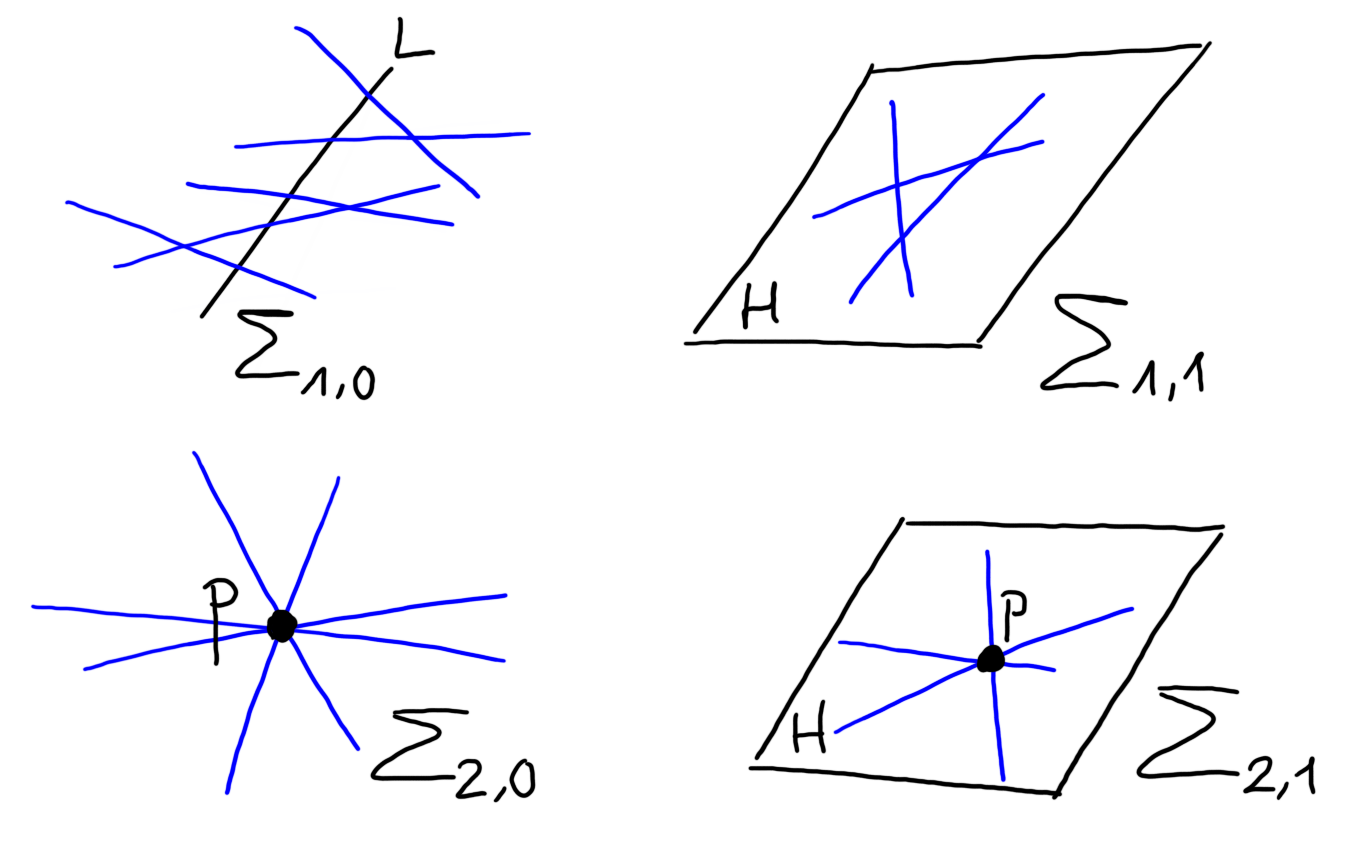
\includegraphics[scale=.75]{pictures/schubertcycles}
\end{figure}

We have the following inclusions:
\begin{center}
    \begin{tikzcd}
	& & \Sigma_{2,0}\arrow[hook]{dr} & & \\
	\{ L\}=\Sigma_{2,2}\arrow[hook]{r} & \Sigma_{2,1}\arrow[hook]{ur}\arrow[hook]{dr} & & \Sigma_{1,0}\arrow[hook]{r} & \Sigma_{0,0}=\mathbb{G}(1,3). \\
	& & \Sigma_{1,1}\arrow[hook]{ur} & & 
    \end{tikzcd}
\end{center}

We define the Schubert cells as
\[ \Sigma_{a,b}^{\circ}=\Sigma_{a,b} \setminus \text{ smaller strata }. \]
Schubert cells define an affine stratification of $\mathbb{G}(1,3)$.
Let us just sketch one part of the proof as an example:

\begin{lm}
    $\Sigma_{1,0}^{\circ}\cong \mathbb{A}^{3}$.
    \begin{proof}
	We have
	\[ \Sigma_{1,0}^{\circ}=\Sigma_{1,0}\setminus (\Sigma_{1,1}\cup \Sigma_{2,0}). \]
	Spelling out the definitions, we see that $\Sigma_{1,0}^{\circ}$ consists of those lines $M$ such that $M\cap L\neq \varnothing$, $p\not\in M$ and $M\not\subseteq H$.
	The idea to show the claimed isomorphism is to fix some $H'\ni p$ with $L\not\subseteq H'$.
	
	\begin{figure}[H]
	    \centering
	    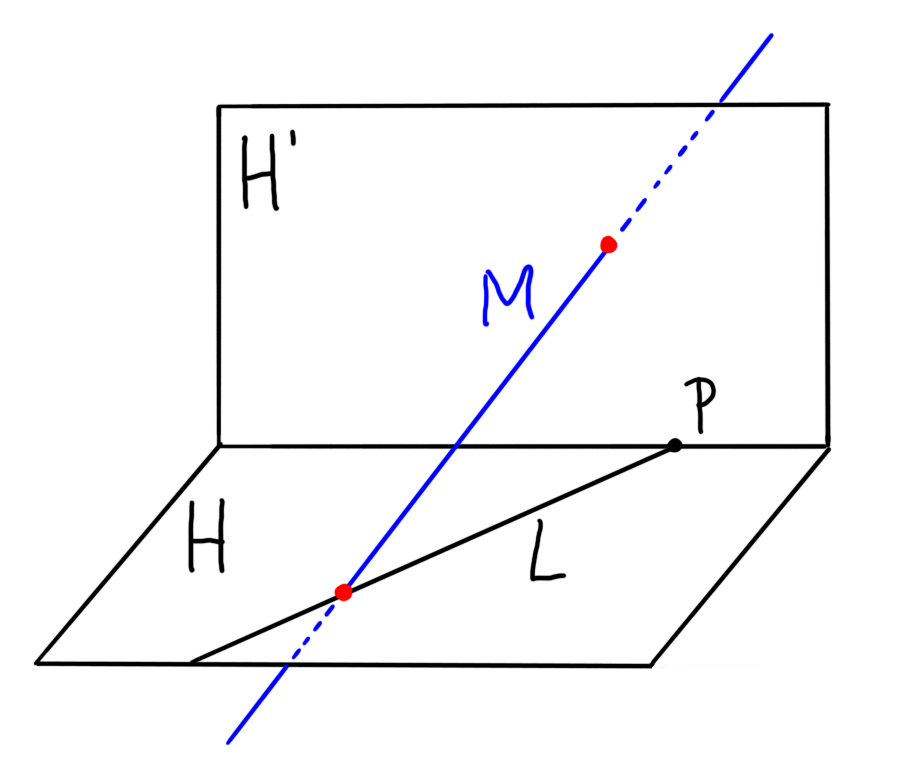
\includegraphics[scale=.75]{pictures/celliso}
	\end{figure}

	Take $M\in \Sigma_{1,0}^{\circ}$; it meets $H'\setminus (H'\cap H)\cong \mathbb{A}^{2}$ in a unique point, and it meets $L\setminus \{ p\}\cong \mathbb{A}^{1}$ in a unique point as well.
	So we define
	\begin{align*}
	    \Sigma_{1,0} & \longmapsto \mathbb{A}^{2}\times\mathbb{A}^{1} \\
	    M & \longmapsto (M\cap H',M\cap L)
	\end{align*}
    \end{proof}
\end{lm}

This stratification of $\mathbb{G}(1,3)$ depends on the chosen flag, but the classes of the closed strata in the Chow ring do not depend on the chosen flag as a consequence of Kleiman's transversality \cite[Theorem 1.7]{eh16}.
Indeed, any two flags $\mathcal{V}$ and $\mathcal{V}'$ are related by a $\operatorname{GL}_{4}$ action, so the Schubert cycles $\Sigma_{a,b}(\mathcal{V})$ and $\Sigma_{a,b}(\mathcal{V}')$ are $\operatorname{GL}_{4}$-translates.
Since $\operatorname{GL}_{4}$ acts transitively on lines in $\mathbb{P}^{3}$, we deduce that $[\Sigma_{a,b}(\mathcal{V})]$ does not depend on the chosen flag.

\section{Fabian Kertels: How many lines intersect 4 random line in space? (27.01.2021)}

\textbf{Goals:}
\begin{itemize}
    \item Compute $A(G(2,4))$ ($3\times $).
    \item Show that the answer to the question in the title is $2$ ($2\times $).
\end{itemize}

In the title, by \textit{random} we mean in general position; and by \textit{space} we mean in $3$-dimensional projective space, say over $\mathbb{C}$ (or at least over an algebraically closed field of characteristic zero).

\subsection{Recap}

\begin{defn}
    For $k\leq \dim(V)=n$, the \textit{Grsassmannian} $G(k,V)$ is defined as the set of $k$-dimensional vector subspaces of $V$ together with the projective variety structure induced by the Pl\"{u}cker embedding:
    \begin{align*}
	G(k,n) & \longrightarrow \mathbb{P}(\wedge^{k} V) \\
	\langle w_{1},\ldots,w_{k}\rangle & \longmapsto [w_{1}\wedge \cdots \wedge w_{k}]
    \end{align*}
    The image of this function consists of the set
    \[ \{[\eta]\mid \operatorname{rk}(V\xrightarrow{(-)\wedge\eta}\wedge^{k+1}V)\leq n-k\}, \]
    which can be described as the vanishing locus of some minors of the corresponding matrix once we fix a basis.
\end{defn}

To compute $A(G(k,v))$, (quasi-affine) stratifications are helpful:

\begin{defn}
    A \textit{stratification} of a variety $X$ is a collection $\{U_{i}\}_{i\in I}$ of irreducible locally closed subvarieties of $X$ with $I$ a finite set and such that
    \[ X=\coprod_{i\in I}U_{i} \quad\text{and}\quad \overline{U_{i}}=\coprod_{U_{j}\subseteq \overline{U_{i}}}U_{j}. \]
\end{defn}

It is an \textit{affine stratification} if for every $i\in I$ there exists some $k_{i}\in \mathbb{N}$ such that $U_{i}\cong \mathbb{A}^{k_{i}}$; and it is a \textit{quasi-affine stratification} if for every $i\in I$ there exists some $k_{i}\in \mathbb{N}$ such that $U_{i}$ is an open subset of $\mathbb{A}^{k_{i}}$.

\begin{prop}
    If $X$ has a quasi-affine stratification $\{ U_{i}\}_{i\in I}$, then $A(X)$ is generated by $\{ [\overline{U_{i}}]\}_{i\in I}$.
\end{prop}

In the case of $\mathbb{G}(1,3)=\mathbb{G}(1,\mathbb{P}^{3})=G(2,4)$ we can produce an affine stratification as follows.
Take a complete flag
\[ \mathcal{V}=\left( \{ p\} \subseteq L\subseteq H\subseteq \mathbb{P}^{3}\right) \]
of $\mathbb{P}^{3}$, and define our closed strata (\textit{Schubert cycles}) as

\begin{itemize}
    \item $\Sigma_{0,0}:=\mathbb{G}(1,3)$;
    \item $\Sigma_{1,0}:=\{ L'\mid L' \cap L\neq \varnothing \}$;
    \item $\Sigma_{2,0}:=\{ L'\mid p\in L'\}$;
    \item $\Sigma_{1,1}:=\{ L'\mid L'\subseteq H\}$;
    \item $\Sigma_{2,1}:=\{ L'\mid p\in L'\subseteq H\}$;
    \item $\Sigma_{2,2}:=\{L\}$.
\end{itemize}

We had the following inclusions
\begin{center}
    \begin{tikzcd}
	& & \Sigma_{2,0}\arrow[hook]{dr} & & \\
	\{ L\}=\Sigma_{2,2}\arrow[hook]{r} & \Sigma_{2,1}\arrow[hook]{ur}\arrow[hook]{dr} & & \Sigma_{1,0}\arrow[hook]{r} & \Sigma_{0,0}=\mathbb{G}(1,3), \\
	& & \Sigma_{1,1}\arrow[hook]{ur} & & 
    \end{tikzcd}
\end{center}

and we defined the \textit{Schubert cells} as $\Sigma_{a,b}^{\circ}=\Sigma_{a,b} \setminus \text{ smaller strata }$.

\begin{cor}
    $A(\mathbb{G}(1,3))$ is generated by the \textit{Schubert classes}
    \[ \sigma_{a,b}:=[\Sigma_{a,b}]. \]
\end{cor}

\subsection{Structure of $A(\mathbb{G}(1,3))$}

\begin{thm}
    We have
    \[ A:=A(\mathbb{G}(1,3))=\oplus_{0\leq b\leq a \leq 2}\mathbb{Z} \sigma_{a,b} \]
    with multiplication given as follows:
    \begin{itemize}
	\item $A^{1}\times A^{1}\to A^{2}\colon \sigma_{1,0}^{2}=\sigma_{1,1}+\sigma_{2,0}$;
	\item $A^{1}\times A^{2}\to A^{3}\colon \sigma_{1,0}\sigma_{1,1}=\sigma_{1,0}\sigma_{2,0}=\sigma_{2,1}$;
	\item $A^{1}\times A^{3}\to A^{4}\colon \sigma_{1,0}\sigma_{2,1}=\sigma_{2,2}$;
	\item $A^{2}\times A^{2}\to A^{4}\colon \sigma_{1,1}^{2}=\sigma_{2,0}^{2}=\sigma_{2,2},\sigma_{1,1}\sigma_{2,0}=0$.
    \end{itemize}
    \begin{proof}
	Since $\mathbb{G}(1,3)$ is proper over $\mathbb{C}$, $A^{4}$ is freely generated by $\sigma_{2,2}$.
	It remains to prove the formulas for the multiplications, since then the group structure would follow.
	For example, suppose we have shown the formulas and we wanted to see that $A^{2}$ is freely generated by $\sigma_{1,1}$ and $\sigma_{2,0}$.
	Let $a,b\in \mathbb{Z}$ such that $a\sigma_{1,1}+b\sigma_{2,0}=0$.
	We can multiply on the left by $\sigma_{1,0}$ to deduce that $a\sigma_{2,2}=0$, hence $a=0$.
	And we can multiply on the left by $\sigma_{1,0}$ to deduce that $b\sigma_{2,2}=0$, hence $b=0$ as well.
	In this way we can decude from the multiplicative formulas that
	\[ A^{2}= \mathbb{Z} \sigma_{1,1}\oplus \mathbb{Z} \sigma_{2,0} \]
	as abelian groups, and with simlar arguments we could do the same for all other degrees.

	To compute the multiplicative formulas we take another flag
	\[ \mathcal{V}'=\left(\{p'\}\subseteq L'\subseteq H'\subseteq \mathbb{P}^{3}\right) \]
	such that $\Sigma_{2,0}\cap \Sigma_{2,0}'$ has dimension $0$, which is possible thanks to Kleiman's transversality.
	Then
	\begin{align*}
	    \sigma_{2,0}^{2} &=|\Sigma_{2,0}\cap \Sigma_{2,0}'|\sigma_{2,2} \\
	     & =|\{ L''\mid p'\in L''\text{ and }p\in L''\}|\sigma_{2,2} \\
	     & = |\{ \overline{pp'}\}|\sigma_{2,2}=\sigma_{2,2}.
	\end{align*}
	And we can argue similarly for the other cases in which the codimensions add up appropriately, namely, for $A^{2}\times a^{2}$ and for $A^{1}\times A^{3}$.

	For $A^{1}\times A^{2}$ we have
	\[ \Sigma_{1,0}\cap \Sigma_{2,0}'=\{ L''\mid p'\in L''\cap L\neq \varnothing, \]
	which is the $(2,1)$-Schubert cycle with respect to a flag containing the point $p'$ and the plane $\overline{p'L}$, so that we have
	\[ \sigma_{1,0}\sigma_{2,0}=\sigma_{2,1}. \]
	In a similar way we deduce that
	\[ \sigma_{1,0}\sigma_{1,1}=\sigma_{2,1}. \]

	It remains to deal with $A^{1}\times A^{1}$.
	From arguments as in the beginning of the proof, we already know that
	\[ A^{2}=\mathbb{Z}\sigma_{1,1}\oplus \mathbb{Z}\sigma_{2,0}. \]
	Therefore it is possible to find $a,b\in \mathbb{Z}$ such that
	\[ \sigma_{1,0}^{2}-a\sigma_{2,0}+b\sigma_{1,1}. \]
	Now
	\begin{align*}
	    a\sigma_{2,2} & = (a\sigma_{2,0}+b\sigma_{1,1})\sigma_{2,0} \\
	    & = \sigma_{1,0}^{2}\sigma_{2,0} \\
	    & = \sigma_{1,0}(\sigma_{1,0}\sigma_{2,0}) \\
	    & = \sigma_{1,0}\sigma_{2,1} = \sigma_{2,2},
	\end{align*}
	so we deduce that $a=1$.
	And likewise we can deduce that $b=1$, finishing the proof.
    \end{proof}
\end{thm}

Now we are ready to answer the question in the title: a line in $\mathbb{P}^{3}$ incident to $m$ lines $L_{1},\ldots,L_{m}$ corresponds to a point in $\mathbb{G}(1,3)$ contained in all the $\Sigma_{1,0}(L_{i})$ for $i\in \{1,\ldots,m\}$.
Here, by $\Sigma_{1,0}(L_{i})$, we mean the Schubert cycle induced by some flag containing $L_{i}$.
So in our case we would compute
\begin{align*}
    |\Sigma_{1,0}(L_{1})\cap \ldots\cap \Sigma_{1,0}(L_{4})| & \overset{(?)}{=} \deg(\sigma_{1,0}^{4}) \\
    & = \deg((\sigma_{1,1}+\sigma_{2,0})^{2}) \\
    & =\deg(2\sigma_{2,2})=2.
\end{align*}

The $(?)$ equality works in this case because Kleiman transversality allows us to apply the moving lemma without generating non-effective cycles in the process and the codimensions fit appropriately.

Alternatively, the multiplication $A^{1}\times A^{1}\to A^{2}$ can also be computed without using associativity.
We would still use the \textit{method of undetermined coefficients}: if $\sigma_{1,0}^{2}\sigma_{2,0}=a\sigma_{2,2}$, then Kleiman's theorem allows us to choose flags $\mathcal{V}$, $\mathcal{V}'$ and $\mathcal{V}''$ in general position, so that
\begin{align*}
    a & = |\{ M\mid M\cap L\neq \varnothing,M\cap L'\neq \varnothing,p''\in M \} | \\
    & = | \{ \overline{p''L}\cap \overline{p''L'}\}| = 1.
\end{align*}

And likewise for the $b$ coefficient.

\subsection{(Static) specialisation}

``Specialise'' $\mathcal{V}$ and $\mathcal{V}'$ enough so that  $\Sigma_{a,b}$ and $\Sigma_{a,b}'$ are still ``general enough'' but at the same time the intersecting can be easily read off.
Using these methods one can give algorithms for computations in Chow rings of general Grassmannians, e.g.~Vakil'06.

We will illustrate this method by computing $\sigma_{1,0}^{2}$ a third time.
Pick flags $\mathcal{V}$ and $\mathcal{V}'$ so that $L\cap L'=\{p\}$ and $H=\overline{L'L}$.
Then, if we knew that the corresponding Schubert cycles $\Sigma_{1,0}$ and $\Sigma_{1,0}'$ were generically transverse, we would be able to deduce
\begin{align*}
    \Sigma_{1,0}\cap \Sigma_{1,0}' & = \{ M \mid M\cap L\neq \varnothing \text{ and }M\cap L'\neq \varnothing\} \\
    & = \{ M\mid M\subseteq H \text{ or } p\in M\} \\
    & = \Sigma_{2,0}\cup \Sigma_{1,1}.
\end{align*}
So we need to check that the two cycles are indeed generically transverse.
First we take some $M\in \Sigma_{2,0}$, i.e.~$p\in M$ and $M\not\in \{L,L'\}$.
We need to compute the tangent spaces of $\Sigma_{1,0}$ and $\Sigma_{1,0}'$ at $M$.
Let $V$ be a $4$-dimensional complex vector space so that our $\mathbb{P}^{3}$ is $\mathbb{P}(V)$.
If $T\subseteq \mathbb{P}^{3}$ is a linear subspace, we denote by $\tilde{T}$ the vector subspace of $V$ such that $T=\mathbb{P}(\tilde{T})$.
Then we have
\[ T_{M}\Sigma_{1,0}=\{ \varphi\in Mor_{\operatorname{Mod}_{\mathbb{C}}}(\tilde{M},V/\tilde{M}) \mid \varphi(\tilde{p})\subseteq \tilde{\overline{ML}}/\tilde{M}\}. \]

This is a $3$-dimensional vector space, and likewise for $T_{M}\Sigma_{1,0}'$.
Therefore both cycles are smooth at $M$, because we saw in the last talk that they are $3$-dimensional cycles with $\Sigma_{1,0}^{\circ}\cong \mathbb{A}^{3}$.
And we also have
\begin{align*}
    T_{M}\Sigma_{1,0}\cap T_{M}\Sigma_{1,0}' & = \{\varphi \mid \varphi(\tilde{p})\subseteq (\tilde{\overline{ML}}\cap \tilde{\overline{ML'}})/\tilde{M} \} \\
    & = \{ \varphi \mid\varphi(\tilde{p})\subseteq \tilde{M}/\tilde{M} \} \\
    & = \{ \varphi \mid \varphi(\tilde{p})=0 \},
\end{align*}
hence the intersection has the expected codimension at $M$.
A similar argument shows the same for $M\in \Sigma_{1,1}$, so the two cycles are indeed generically transverse.

\subsection{A geometric picture}

Brief discussion following \cite[\S 3.4.1]{eh16}.

\section{Luca Terenzi: Knutson--Tao puzzles and Chern classes (03.02.2021)}
Notation: $k$ an algebraicallly closed field of characteristic $0$ (e.g.~$k = \mathbb{C}$).

\subsection{Knutson--Tao puzzles}

Main character: $\mathbb{G}(1,3) = G(2,4)$, the Grassmannian of lines in $\mathbb{P}^{3}$.
Recall from the last talk that the Chow ring $A(G(2,4))$ is freely generated as a graded abelian group by the Schubert classes
\[ \sigma_{a,b} = [ \Sigma_{a,b}(\mathcal{V}) ] \in A^{a+b} \]
for $2 \geq a \geq b \geq 0$.
They satisfy the relation
\[ \sigma_{1}^{2} = \sigma_{1,0}^{2} = \sigma_{1,1} + \sigma_{2,0} \]
in $A^{2}$.
We established it in $2$ different ways:

\begin{enumerate}
  \item With the method of undetermined coefficients.
    Write $\sigma_{1,0}^{2} = a\sigma_{1,1} + b\sigma_{2,0}$ for some $a,b \in \mathbb{Z}$.
    Then determine $a$ and $b$ by multiplying this relation with suitable classes (i.e.~$\sigma_{2,0}$, $\sigma_{1,1}$).
  \item By static specialization.
    Choose two complete flags $\mathcal{V}$ and $\mathcal{V}'$ so that
    \begin{enumerate}[label=(\roman*)]
      \item the cycles $\Sigma_{1,0}(\mathcal{V})$ and $\Sigma_{1,0}(\mathcal{V}')$ intersect generically transversely, and
      \item the intersection $\Sigma_{1,0}(\mathcal{V}) \cap \Sigma_{1,0}(\mathcal{V}')$ can be easily described geometrically.
    \end{enumerate}
    Then compute $[\Sigma_{1,0}(\mathcal{V})] \cdot [\Sigma_{1,0}(\mathcal{V}')] = [\Sigma_{1,0}(\mathcal{V}) \cap \Sigma_{1,0}(\mathcal{V}')]$.
\end{enumerate}

\begin{rem}
  In both cases, one cannot avoid giving an explicit geometric interpretation to some products of Schubert classes.
  Doing the same in general (i.e.~for $G(r,n)$ with $r,n \gg 0$) seems really difficult.
\end{rem}

Knutson--Tao puzzles allow us to compute products of general Schubert clases in a purely combinatorial way!

But first, let us change the notation for Schubert classes a little bit.
Let $V$ be a $k$-vector space of dimension $n \geq 0$, and let $r \leq n$ be a natural number.
Consider $G(r,V) \cong G(r,n)$.
Fix a complete flag $\mathcal{V}$ given by subspaces
\[ 0 = V_{0} \subset V_{1} \subset \ldots \subset V_{n} = V \]
with $\dim(V_{i}) = i$.
Then, to every $r$-tuple
\[ a = (a_{1}, \ldots, a_{r}) \in \mathbb{N}^{r} \]
with $n - r \geq a_{1} \geq \ldots \geq a_{r} \geq 0$ we associate the Schubert cycle $\Sigma_{a}(\mathcal{V})$ given by the set
\[ \{ W \in G(r,n) \mid \dim(V_{n-r+i-a_{i}} \cap W) \geq i \text{ for all }i \}. \]
Geometric intuition: for a general $W \in G(r,n)$, we have
\[ \dim(V_{n-r+j} \cap W) = \begin{cases}
  0, & j < 0 \\
  j, & j\geq 0.
\end{cases} \]
Hence we have $W \in \Sigma_{a}(\mathcal{V})$ if and only if the condition $\dim(V_{n-r+j} \cap W) \geq i$ is satisfied at least $a_{i}$ steps earlier than expected.
Equivalently, for $W \in G(r,n)$ consider the sequence of subspaces of $W$ given by $\mathcal{V} \cap W$, that is,
\[ 0 = (V_{0} \cap W) \subset (V_{1} \cap W) \subset \ldots \subset (V_{n} \cap W) = W. \]
At each step, the dimension increases by $0$ or $1$; since $\dim(W) = r$, it increases by $1$ exactly $r$ times.
We can encode this into an $n$-string
\[ \alpha = \alpha_{W} = (\alpha_{1}, \ldots, \alpha_{n}) \in \{ 0, 1\}^{n} \]
such that $\sum_{i} \alpha_{i} = r$, and the cycle $\Sigma_{a}(\mathcal{V})$ is the closure of the locus
\[ \{ W \in G(r,n) \mid \alpha_{j} = 1 \Leftrightarrow \exists i,, j = n - r + i - a_{i} \}. \]
Summary: the sequence $a = (a_{1}, \ldots, a_{r})$ corresponds to a unique $n$-string $\alpha = (\alpha_{1}, \ldots, \alpha_{n})$ as above.
Hence we can write
\[ \Sigma_{a}(\mathcal{V}) = S_{\alpha}(\mathcal{V}), \quad \sigma_{a} = s_{\alpha}. \]

\begin{exmp}
  In $A(G(2,4))$ we have $\sigma_{1,0} = s_{(0,1,0,1)}$, $\sigma_{1,1} = s_{(0,1,1,0)}$ and $\sigma_{2,0} = s_{(1,0,0,1)}$.
  The relation $\sigma_{1,0}^{2} = \sigma_{1,1} + \sigma_{2,0}$ becomes
  \[ s_{(0,1,0,1)}^{2} = s_{(0,1,1,0)} + s_{(1,0,0,1)}. \]
  We will re-prove this relation soon.
\end{exmp}

\begin{defn}
  Consider the following $3$ types of pieces:
  \begin{itemize}
    \item 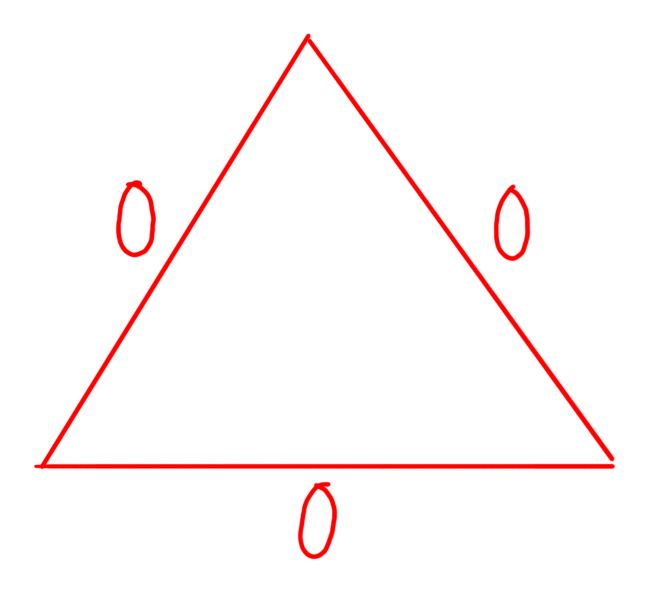
\includegraphics[scale=.2]{pictures/triangle0} $0$-triangle,
    \item 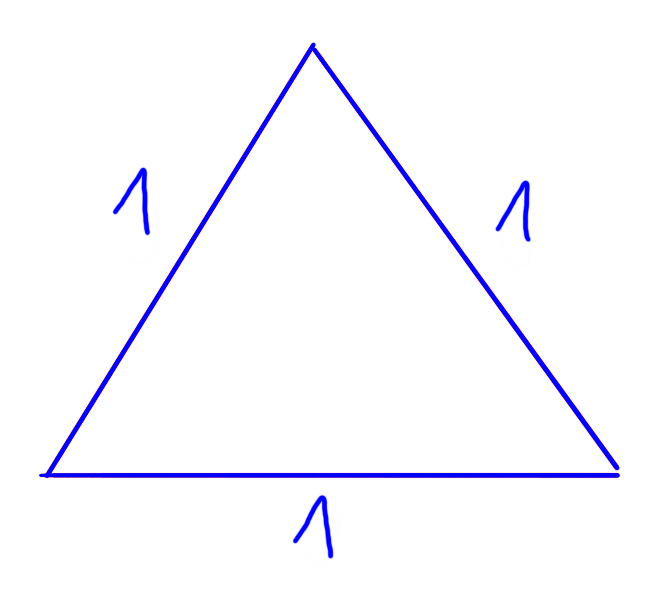
\includegraphics[scale=.2]{pictures/triangle1} $1$-triangle, and
    \item 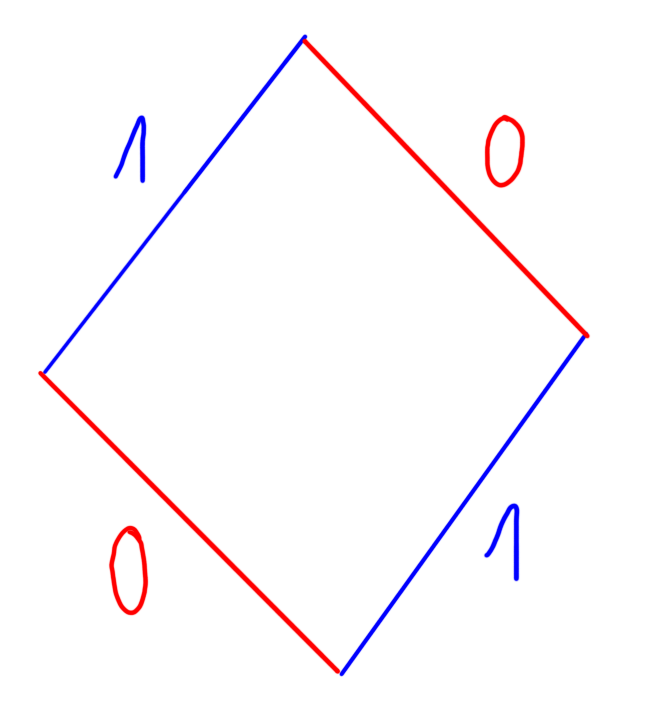
\includegraphics[scale=.2]{pictures/rhombus} rhombus.
  \end{itemize}
  A \textit{Knutson--Tao puzzle} of size $n \in \mathbb{N}$ is a decomposition of a lattice triangle of side-length $n$ into lattice polygons such that
  \begin{itemize}
    \item all edges are labelled \color{red}$0$ \color{black} or \color{blue}$1$\color{black}, and
    \item every region is a puzzle piece as above.
  \end{itemize}
\end{defn}

\begin{exmp}
  Some valid Knutson--Tao puzzles would be
  \begin{figure}[H]
    \centering
    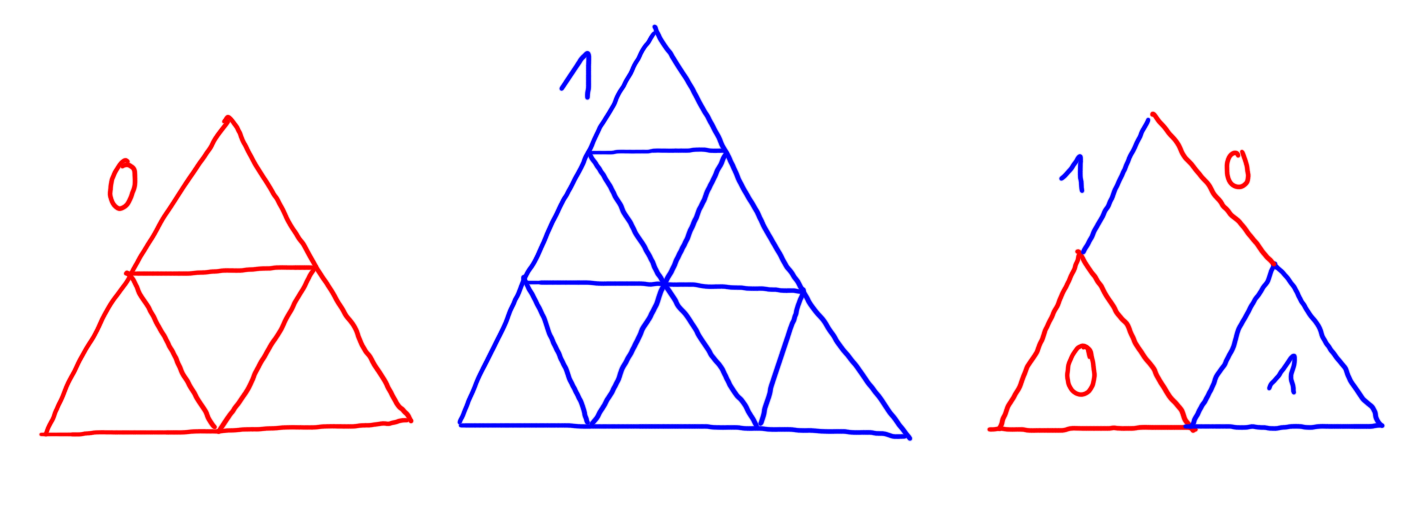
\includegraphics[scale=.7]{pictures/knutsontaoexmp}
  \end{figure}
\end{exmp}

Knutson--Tao puzzles compute products of Schubert classes on Grassmannians:

\begin{thm}
  Given two $n$-strings $\alpha,\beta \in \{0, 1\}^{n}$ with $\sum_{i} \alpha_{i} = \sum_{i} \beta_{i} = r$, write in $A(G(r,n))$
  \[ s_{\alpha}\cdot s_{\beta} = \sum_{\gamma} m_{\alpha\beta}^{\gamma} s_{\gamma} \]
  for some integers $m_{\alpha\beta}^{\gamma} \in \mathbb{Z}$.
  Then
  \begin{figure}[H]
    \centering
    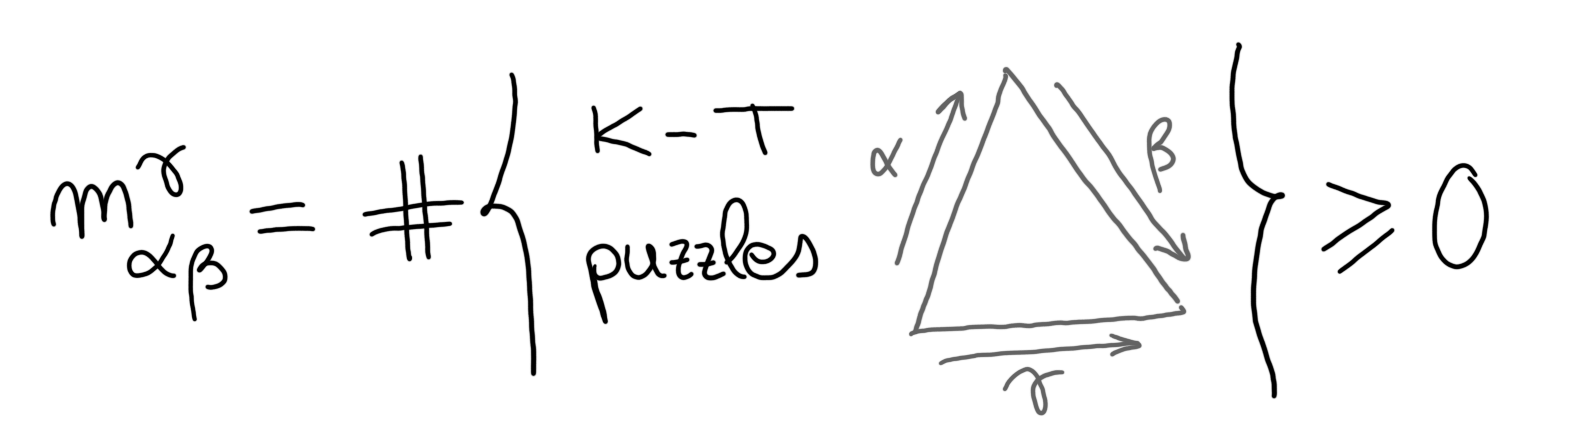
\includegraphics[scale=.7]{pictures/knutsontaocoefficients}
  \end{figure}
\end{thm}

\begin{rem}
  The coefficients $m_{\alpha\beta}^{\gamma}$ are well-defined.
\end{rem}

\begin{exmp}
  We compute $\sigma_{1,0}^{2} = s_{(0,1,0,1)}^{2}$ using Knutson--Tao puzzles:
  \begin{figure}[H]
    \centering
    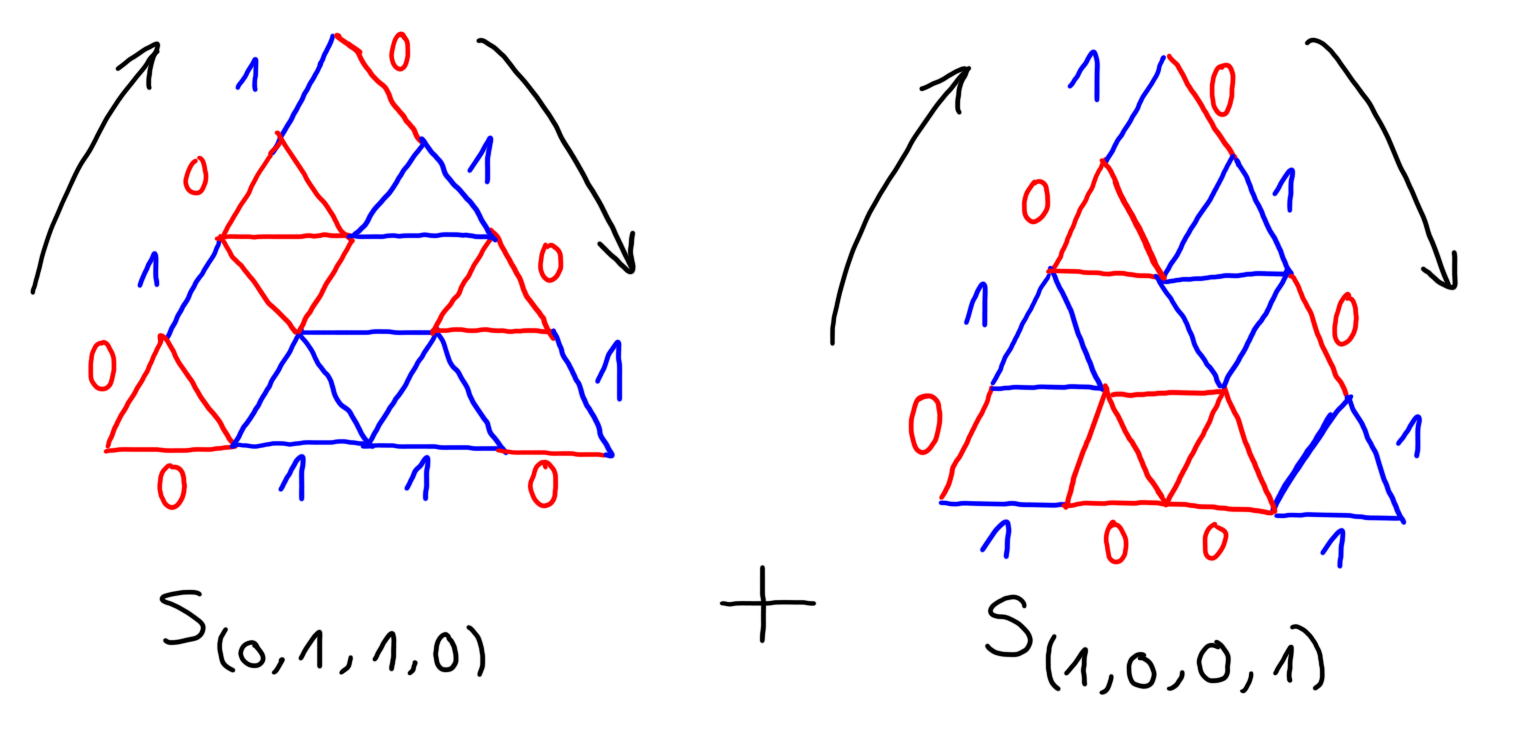
\includegraphics[scale=.7]{pictures/knutsontaosum}
  \end{figure}
\end{exmp}

The previous theorem allows us to derive some general symmetries of Schubert calculus:

\begin{cor}
  With the same notation as in the theorem, we have the following relations:
  \begin{enumerate}[label=(\roman*)]
    \item Rotation: $m_{\alpha^{\vee}\beta^{\vee}}^{\gamma} = m_{\beta^{\vee}\gamma^{\vee}}^{\alpha} = m_{\gamma^{\vee}\alpha^{\vee}}^{\beta}$, where $\alpha_{i}^{\vee} := \alpha_{n - i}$.
    \item Reflection: $m_{\alpha\beta}^{\gamma} = m_{\bar{\beta}\bar{\alpha}}^{\bar{\gamma}}$, where $\bar{\alpha}_{i} := 1 - \alpha_{n - i}$.
  \end{enumerate}
\end{cor}

\subsection{Introduction to Chern classes}

Main characters: $X$ a smooth connected $k$-variety and $\mathscr{E}$ a rank $r$ vector bundle on $X$ (=locally free sheaf of $\mathscr{O}_{X}$-modules of rank $r$).

Many interesting subvarieties $Y \subseteq X$ can be written as:

\begin{itemize}
  \item Vanishing locus of a family of sections of $\mathscr{E}$.
  \item Degeneracy locus of a collection of sections of $\mathscr{E}$ (i.e.~locus where they are linearly dependent).
\end{itemize}

These subvarieties can be studied systematically with the theory of Chern classes, which allows us to translate questions of intersection theory into questions of linear algebra.

\subsection{The  first Chern class of a line bundle}

Let $\mathscr{L}$ be a line bundle on $X$.
A reational section $\sigma \in \Gamma(X, \mathscr{L} \otimes_{\mathscr{O}_{X}} \mathscr{K}_{X})$ (where $\mathscr{K}_{X}$ is the constant sheaf of rational functions) defines a Cartier divisor $D_{\sigma}$ as follows.
Choose $U \subseteq X$ a non-empty Zariski-open subset such that $\mathscr{L}|_{U} \cong \mathscr{O}_{U}$.
We can then write $\sigma_{U} = f_{U} / g_{U}$ for some $f_{U}, g_{U} \in \mathscr{O}_{X}(U)$.
Define $(D_{\sigma})|_{U} := \operatorname{div}(f_{U}) - \operatorname{div}(g_{U})$.
Then glue these objects to a divisor $D_{\sigma}$ on $X$.
Given another rational section $\tau$ of $\mathscr{L}$, we have $\sigma = f \tau$ for some $f \in K(X) = \Gamma(X, \mathscr{K}_{X})$, and so $D_{\sigma} = \operatorname{div}(f) + D_{\tau}$, which implies that
\[ D_{\sigma} = D_{\tau} \]
in $A^{1}$.

\begin{defn}
  The element $c_{1}(\mathscr{L}) := [D_{\sigma}] \in A^{1}(X)$ is called the \textit{first Chern class} of $\mathscr{L}$.
\end{defn}

\subsection{Axiomatic definition of Chern classes}

More generally, for every vector bundle $\mathscr{E}$ on $X$ it is possible to define classes $c_{i}(\mathscr{E}) \in A^{i}(X)$ for all $i \geq 0$ satisfying many useful properties:

\begin{thm}
  There is a unique way of assigning to every smooth variety $X$ and every vector bundle $\mathscr{E}$ on $X$ a class
  \[ c(\mathscr{E}) = 1 + c_{1}(\mathscr{E}) + c_{2}(\mathscr{E}) + \ldots \in A(X) \]
  with $c_{i}(\mathscr{E}) \in A^{i}(X)$, so that:
  \begin{enumerate}[label=(\roman*)]
    \item if $\mathscr{L}$ is a line bundle on $X$, then
      \[ c(\mathscr{L}) = 1 + c_{1}(\mathscr{L}), \]
      where $c_{1}(\mathscr{L})$ is the class defined before;
    \item given global sections $\tau_{0}, \ldots, \tau_{r-i} \in \Gamma(X,\mathscr{E})$ such that the locus $D \subseteq X$ where they are linearly dependent has codimension $i$, then
      \[ c_{i}(\mathscr{E}) = [D] \in A^{i}(X); \]
    \item for every short exact sequence of vector bundles
      \[ 0 \to \mathscr{E}' \to \mathscr{E} \to \mathscr{E}'' \to 0 \]
      we have \textit{Whitney's formula}:
      \[ c(\mathscr{E}) = c(\mathscr{E}') \cdot c(\mathscr{E}''); \]
    \item for every morphism of smooth varieties $\varphi \colon Y \to X$ we have
      \[ \varphi^{*}c(\mathscr{E}) = c(\varphi^{*}\mathscr{E}). \]
  \end{enumerate}
\end{thm}

\begin{defn}
  We call
  \begin{itemize}
    \item $c(\mathscr{E}) \in A(X)$ the \textit{total Chern class} of $\mathscr{E}$, and
    \item $c_{i}(\mathscr{E}) \in A^{i}(X)$ the \textit{$i$-th Chern class} of $\mathscr{E}$.
  \end{itemize}
\end{defn}

\begin{cor}\label{cor:filtration}
  If $\mathscr{E}$ is a vector bundle on $X$ admitting a filtration
  \[ 0 = \mathscr{E}_{0} \subset \mathscr{E}_{1} \subset \ldots \subset \mathscr{E}_{n} = \mathscr{E} \]
  by subvector bundles $\mathscr{E}_{i}$ such that the corresponding quotients
  \[ \mathscr{L}_{i} := \mathscr{E}_{i} / \mathscr{E}_{i+1} \]
  are again vector bundles, then
  \[ c(\mathscr{E}) = \prod_{i=1}^{n} c(\mathscr{L}_{i}) = c\left(\oplus_{i=1}^{n}\mathscr{L}_{i}\right). \]
\end{cor}

\subsection{The splitting principle}

\begin{lm}[Splitting construction]\label{lm:splitting}
  Let $X$ be a smooth connected variety and $\mathscr{E}$ a vector bundle on $X$.
  Then there exist a smooth connected variety $Y$ and a morphism $\varphi \colon Y \to X$ such that:
  \begin{enumerate}[label=(\roman*)]
    \item the map $\varphi^{*} \colon A(X) \to A(Y)$ is injective, and
    \item the vector bundle $\varphi^{*}\mathscr{E}$ on $Y$ admits a filtration
      \[ 0 = \mathscr{E}_{0} \subset \mathscr{E}_{1} \subset \ldots \subset \mathscr{E}_{r} = \varphi^{*}\mathscr{E} \]
      by subvector bundles $\mathscr{E}_{i}$ such that every quotient $\mathscr{L}_{i} := \mathscr{E}_{i} / \mathscr{E}_{i+1}$ is a line bundle.
  \end{enumerate}
  \begin{proof}
    (Sketch) We construct $Y$ by induction on $r = \operatorname{rk}(\mathscr{E})$.
    If $r \in \{0,1\}$, then there is nothing to show.
    If $r \geq 2$, then define $Y_{1} := \mathbb{P}(\mathscr{E}) \xrightarrow{\pi} X$.
    Then $\pi^{*}\mathscr{E}$ contains the tautological subbundle $\mathscr{S} \subseteq \pi^{*}\mathscr{E}$, giving a short exact sequence of vector bundles
    \[ 0 \to \mathscr{S} \to \pi^{*}\mathscr{E} \to \mathscr{Q} \to 0. \]
    Moreover, $\pi^{*} \colon A(X) \to A(Y_{1})$ is injective.
    Now replace $(X,\mathscr{E})$ by $(Y_{1},\mathscr{Q})$...
  \end{proof}
\end{lm}

\begin{cor}[Splitting principle]
  Every identity between combinations of Chern classes holds for all vector bundles as soon as it holds for those which are direct sums of line bundles.
  \begin{proof}
    Combine \Cref{lm:splitting} and \Cref{cor:filtration}.
  \end{proof}
\end{cor}

\begin{exmp}
  We have the following identities:
  \begin{enumerate}
    \item If $\mathscr{E}$ is a vector bundle of rank $r$, then
      \[ c_{i}(\mathscr{E}) = 0 \text{ for all } i > r. \]
    \item If $\mathscr{E}^{\vee}$ is the dual bundle of $\mathscr{E}$, then
      \[ c_{i}(\mathscr{E}^{\vee}) = (-1)^{r}c_{i}(\mathscr{E}). \]
    \item If $\det(\mathscr{E}) := \bigwedge^{r}\mathscr{E}$ is the determinant line bundle, then
      \[ c_{1}(\det(\mathscr{E})) = c_{1}(\mathscr{E}). \]
    \item If $\mathscr{E}_{i}$ has rank $r_{i}$ for $i \in \{1,2\}$, then
      \[ c_{1}(\mathscr{E}_{1} \otimes \mathscr{E}_{2}) = r_{2}c_{1}(\mathscr{E}_{1}) + r_{1}c_{1}(\mathscr{E}_{2}). \]
  \end{enumerate}
\end{exmp}

\bibliographystyle{alpha}
\bibliography{main}
\vfill

\end{document}
